\documentclass[a4paper, 11pt]{memoir}

% Nécessaire
\usepackage[utf8]{inputenc}
\usepackage[T1]{fontenc}
\usepackage{lmodern}

% Biblio
\usepackage{natbib}
\bibliographystyle{abbrvnat}
\usepackage{hypernat}
\bibpunct{\textcolor{blue}{[}}{\textcolor{blue}{]}}{\textcolor{blue}{;}}{a}{\textcolor{blue}{,}}{;}

\usepackage[french]{babel}
\usepackage{amsmath, amsthm}
\usepackage{amsfonts,amssymb}

\usepackage[colorlinks=true, citecolor=blue, linkcolor=., urlcolor = blue]{hyperref}

% Marge
\usepackage{geometry}
\geometry{margin={3cm, 3cm}}
% \usepackage[inner=3cm,outer=2cm]{geometry}
% \usepackage[inner=100pt, textwidth=400pt]{geometry}

% Figures, graphiques
\usepackage{graphicx}
\usepackage{epsfig}
% \usepackage{caption}
\usepackage{wrapfig}
% \usepackage{graphics}
\usepackage{wrapfig}
\usepackage{afterpage}
\usepackage{adjustbox}

\usepackage[graphicx]{realboxes}
% Surlignage
\usepackage{alltt}

% Couleurs
\usepackage[dvipsnames]{xcolor}
\usepackage{soul}
\usepackage{color}
\usepackage{colortbl}

% Indicatrice
\usepackage{dsfont}
\usepackage{textcomp}

\usepackage{multirow}
\usepackage{eurosym}
\usepackage{extarrows}

% Graphique
\usepackage{tikz}

\usepackage{enumitem}
% Thème, style
\usepackage{lettrine}
\usepackage{titlesec}
\renewcommand{\chapnumfont}{%     % define font for chapter number
  \usefont{T1}{pnc}{b}{n}%      % choose New Chancery, bold, normal shape
  \fontsize{100}{100}%          % font size 100pt, baselineskip 100pt
  \selectfont%                  % activate font
}
\colorlet{chapnumcol}{gray!75}  % color for chapter number

\titleformat{\chapter}[display]
{\filleft\bfseries}
{\filleft\chapnumfont\textcolor{chapnumcol}{\thechapter}}
{-24pt}
{\Huge}
\usepackage{titletoc}
\usepackage{fancyhdr}
 \usepackage{pdflscape}
\pagestyle{plain}
\usepackage[colorlinks=true, citecolor=blue, linkcolor=., urlcolor = blue]{hyperref}
\usepackage{adjustbox}
\usepackage{pdfpages}

\begin{document}

\frontmatter

% \includepdf{garde_iae.pdf}
% Page de garde
% \hypersetup{pageanchor=false}

\begin{titlingpage}
\epsfig{file = plots/logo_fds3.eps, scale = 0.35}


\vspace*{2.5cm}

\begin{center}
 
 {\large \textsc{Master de Mathématiques de l'INformation et de la Décision}}


 \vspace*{2cm}
 
 
 {\Large \textbf{Modélisation du système manguier~--~cécidomyies des fleurs pour une évaluation de modes de gestion du ravageur et de ses dégâts}}
 \vspace*{1cm}
 
 Bastien Reyné
 
\end{center}

\vspace*{2cm}

\noindent
\begin{tabular}{ll}
Encadré par : & Isabelle Grechi (Cirad, UPR HortSys)\\
 & Frédéric Boudon (Cirad, UMR AGAP)
\end{tabular}

\vspace*{2cm}

\begin{center}
 \epsfig{file = plots/logo_cirad2.eps, scale = 0.20}
\end{center}



\vfill

\begin{center}
 Année universitaire 2018/2019
\end{center}


\end{titlingpage}

% \hypersetup{pageanchor=true}

\begin{abstract}
Le manguier est un arbre fruitier qui a une floraison étalée dans le temps.
Cela produit des conditions favorables au développement des ravageurs, dont la cécidomyie des fleurs qui s'attaque aux inflorescences et fait donc beaucoup de dégâts sur la production.
Une expérimentation a été menée sur des vergers en 2017 pour tester différentes modalités de couverture du sol (car la cécidomyie se développe en partie dans le sol).
L'acquisition de données est cependant difficile, la cécidomyie étant un insecte volant ; les données disponibles quantifient donc le nombre de larves s'éjectant des inflorescences.
À partir de ces données et des connaissances présentes dans la littérature, un modèle décrivant la dynamique de population de cécidomyie des fleurs à différents stades (larves et adultes) en fonction de la dynamique de population d'inflorescences a été établi sous la forme d'équations.
Il prend en compte les différentes étapes du cycle de développement de la cécidomyie des fleurs : ponte des œufs, développement larvaire, enfouissement des larves dans le sol, phase de pupaison et émergence des adultes dans le verger.
Le modèle a été calibré avec un algorithme génétique multicritères (NSGA-II) et les solutions optimales ont été analysées.
Ce modèle a permis de recréer les dynamiques de larves capturées de manière convaincante.
Le modèle semble aussi indiquer que les cécidomyies sont soumises à un phénomène de saisonnalité, autre que l'absence de ressources ou un changement de température, qui met un terme à leur prolifération en fin de saison.
\end{abstract}

\chapter*{Remerciements}
\addcontentsline{toc}{chapter}{Remerciements} 
\thispagestyle{empty}

Merci !



\tableofcontents

\mainmatter

% Chapitre 1
\chapter{Introduction}

\lettrine{L}{e} Cirad --- où j'ai effectué mon stage --- est un organisme de recherche spécialisé dans l'agronomie des régions tropicales et subtropicales, et l'un de ses objectif principal est d'encourager le développement durable desdites régions.
Cependant la notion de développement durable vient avec quelques contraintes.
Notamment, la durabilité implique la limitation des pesticides; et le développement induit la nécessité d'une production agricole efficiente, capable de nourrir dix milliards de personnes d'ici 2050.
L'une des missions du Cirad est de trouver des alternatives aux pesticides afin de gérer les bioagresseurs qui sont responsables de dégâts sur les cultures et engendrent des pertes de production.

Ainsi, il est naturel que le sixième fruit le plus produit au monde, à savoir la mangue\footnote{La sixième production fruitière mondiale est en réalité le groupement des mangues, mangoustans et goyaves \citep{fao}}, soit l'objet de recherches visant à rendre sa culture plus durable.
C'est d'autant plus vrai que la culture du manguier (\emph{Mangifera indica L.}) n'est pas toujours facile.
En effet, les manguiers présentent de forts asynchronismes phénologiques, que ce soit à l'intérieur d'une même parcelle entre les différents arbres ou à l'intérieur même d'un arbre entre les différentes branches.
Cela entraîne une floraison et une fructification étalée dans le temps, rendant la gestion des vergers plus difficile.
Ce phénomène entraîne aussi, pour les fleurs et les fruits, une fenêtre d'exposition prolongée aux bioagresseurs, ce qui favorise leur prolifération.
Et ils sont légion.
On peut citer la cécidomyie des fleurs et la mouche des fruits chez les ravageurs ou encore l'oïdium et l'anthracnose, des maladies fongiques.
% Synchroniser la floraison --- à travers l'élagage --- réduirait la fenêtre d'exposition aux ravageurs et \emph{a fortiori} diminuerait leur nombre.

Parmi ces ravageurs, la cécidomyie des fleurs (\emph{Procontarinia mangiferae}) peut fortement impacter la production.
Cette dernière pond ses œufs dans les inflorescences où elle réalise une partie de son cycle de développement, la fin du cycle se déroulant dans le sol.
Le développement des larves dans les inflorescences provoque des dommages potentiellement importants voire la mort des inflorescences. 
Et qui dit pas d'inflorescences, dit pas de mangues !
Dans le contexte de développement durable, il s'agit donc de trouver des solutions alternatives aux pesticides pour gérer ce ravageur et ses dégâts.

% Une partie du cycle de développement de la cécidomyie a lieu dans le sol, on peut envisager différents recouvrements du sol (par exemple, une bache) qui permettraient de stopper le cycle de développement du ravageur.
% Il est aussi envisagé de réduire la fenêtre d'exposition des inflorescences aux cécidomyies en synchronisant la floraison.
% On propose par la suite un modèle pour mieux appréhender les intéractions entre les cécidomyies et les manguiers.
% Ce modèle devrait permettre de tester des modes de conduites des vergers \emph{in silico} afin de voir si l'on peut fortement diminuer la population de cécidomyies sans utiliser d'intrants phytosanitaires.

Pour ce faire, deux pistes sont envisagées.
La première serait la synchronisation de la floraison, grâce à des pratiques culturales appropriées (la taille, par exemple), ce qui réduirait la fenêtre d'exposition des inflorescences aux ravageurs et limiterait par conséquent leur nombre, en limitant le nombre de cycle de développement du ravageur à l'intérieur du verger.
%La seconde repose sur le fait que l'une des phases du cycle de développement de la cécidomyie a lieu dans le sol.
La seconde repose sur le fait qu'une partie du cycle de développement du ravageur se passe dans le sol.
Restreindre l'accès au sol (\emph{e.g.} avec un enherbement haut, qui augmente le trajet des larves pour atteindre la terre et favorise la présence de prédateurs) ou l'empêcher (\emph{e.g.} en utilisant une bâche) permet d'altérer ou rompre le cycle de développement du ravageur, et devrait \emph{a priori} permettre de réduire sa présence. 
% Ainsi, empêcher une cécidomyie d'entrer dans le sol devrait \emph{a priori} permettre de réduire la présence de ces ravageurs.
Afin de pouvoir vérifier cette hypothèse, une expérimentation sur un verger a été conduite en 2017 ; une parcelle a été divisée en trois sous-parcelles pour tester trois modalités de couverture du sol différentes : un enherbement ras, un paillage synthétique et un enherbement haut. 
De cette expérimentation, des données ont été acquises.
Pour aller plus loin dans la compréhension du fonctionnement du système manguier -- cécidomyies des fleurs et de sa gestion par les deux pistes envisagées, une démarche de modélisation de ce système a été engagée.
Une première version du modèle a été réalisée lors du stage de \citet{laurie}.
Mon stage en est la suite et a pour objectifs :
\begin{enumerate}
 \item modéliser le système manguier -- cécidomyies des fleurs, en utilisant les données expérimentales pour le calibrer ;
 \item analyser le fonctionnement du système manguier -- cécidomyies des fleurs ;
 \item tester \emph{in silico} l'effet de la dynamique de floraison et de conditions environnementales, telles que la pression exogène du ravageur, sur l'infestation du verger par les cécidomyies des fleurs.
\end{enumerate}




[BALANCER LE PLAN]


% Chapitre 2
\chapter{Connaissances biologiques} 

\lettrine{O}{n} s'intéresse dans ce chapitre aux manguiers et aux cécidomyies des fleurs.
On s'intéresse en particulier à leurs descriptions d'un point de vue biologique, leurs développements et leurs intéractions.
Autrement dit, on recence ici les connaissances biologiques nécessaires à la compréhension de notre sujet.


\section{Les manguiers}

Le manguier est un arbre qui a une croissance végétative rythmique.
Cela signifie que sa croissance est entrecoupée par des périodes de repos.
Durant les périodes de croissance, les branches sont prolongées par des tiges qui ont des feuilles.
Ces tiges sont appelées \emph{unités de croissance}. 
Si une unité de croissance prolonge la branche dans l'axe, alors elle est dite apicale ; si elle la prolonge sur le côté, elle sera qualifiée de latérale.
Au fil du temps, les unités de croissance perdent leurs feuilles, durcissent et grossissent jusqu'à faire partie intégrante de la branche.
On peut alors voir le manguier comme un empilement d'unités de croissance;
la base du tronc étant l'unité de croissance la plus ancienne et celles qui portent des feuilles les plus récentes \citep{normand2009}.
Des unités de croissance sont visibles sur la figure~\ref{fig:uc}.
\begin{figure}[ht]
 \centering
 \epsfig{file = photos/uc.eps, scale = 0.09}
 \caption{Photographie d'une branche portant des unités de croissance.}
 \label{fig:uc}
\end{figure}

Et ce sont ces unités de croissance qui portent les \emph{inflorescences}.
Les inflorescences désignent des groupements de bourgeons. 
Ces bourgeons deviennent des fleurs qui elles-même deviennent des fruits, si elles sont fécondées.
En théorie.
En pratique, les bourgeons ne survivent que rarement jusqu'au stade de fruit, ils meurent bien souvent avant.
S'ils meurent parfois à cause des conditions climatiques, la principale raison de leurs morts restent les attaques des ravageurs.

La forte présence des ravageurs s'explique en grande partie par le \emph{cycle phénologique} du manguier.
On désigne par cycle phénologique les phénomènes périodiques qui rythment le monde vivant en fonction des variations climatiques.
Et il y a chez le manguier, en sus des conditions climatiques, d'autres facteurs qui influent sur la phénologie tels que la position de l'unité de croissance ou la charge en fruit de l'année précédente \citep{magne2004effet, normand2009axis}.
Il en résulte que le cycle phénologique est très variable d'un manguier à l'autre.
On observe même des différences au niveau phénologique entre les différentes unités de croissance d'un même arbre.
Mais cela implique aussi que le cycle phénologique peut être modifié (dans une certaine mesure) grâce à des opérations techniques, comme la taille par exemple.

Du cycle phénologique viennent les \emph{stades phénologiques} des inflorescences.
Ils caractérisent le niveau de développement des inflorescences.
On considère ici les stades phénologiques allant de C à F.
Le stade C correspond au débourrement (l'éclosion des bourgeons) de l'inflorescence.
Le stade F s'étend entre l'apparition de la première fleur jusqu'à la disparition de la dernière.
Et les stades D et E représentent les étapes intermédiaires du développement qui mènent du débourrement à la floraison.
Les durées des stades phénologiques sont les suivantes :
\begin{center}
\begin{tabular}{llll}
Stade phénologique & C/D & E & F\\
Durée (en jours) & 7 & 9 & 34
\end{tabular}
\end{center}
Les inflorescences ont ainsi une durée de vie théorique de 50 jours \citep{laurie}. Cette durée théorique peut être réduite en cas d'attaque de cécidomyies des fleurs, surtout lorsque l'inflorescence se fait attaquer lors des premiers stades, moment où l'inflorescence est la plus vulnérable.

La saison des mangues a lieu pendant l'hiver (austral).







\section{Les cécidomyies des fleurs}


% Chapitre 3
\chapter{Données expérimentales disponibles} 

\lettrine{C}{e} chapitre explique l'expérimentation qui a été menée en 2017 sur deux vergers dans la commune de Saint-Paul (à la Réunion). 
On décrira le dispositif de l'expérimentation et les données qui en ont étés acquises.
Le but de cette expérimentation était de déterminer quel est l'impact de la modalité de couverture du sol dans le degré d'infestation d'un verger.


\section{Dispositif expérimental et suivis}

Le verger expérimental (que l'on apellera aussi parcelle par la suite) n\textdegree1 a une superficie de 0.33 hectares et est séparé en trois sous-parcelles comprenant chacune trente arbres [À CHECKER].
Sur chacune des trois sous-parcelle, une modalité de couverture du sol différente est mise en place.
Sur un côté il y avait un enherbement entretenu de sorte qu'il reste ras, la modalité \emph{enherbement ras (ER)} fera référence à ce traitement dans la suite du document.
La sous-parcelle du milieu fut baché, afin que les cécidomyies ne puissent ni entrer dans le sol ni en sortir ; cette modalité correspond au \emph{paillage synthétique (PS)}. 
La dernière partie fut laissée telle quelle, sans entretien particulier, donnant ainsi un \emph{enherbement haut (EH)}.
À noter qu'à côté de ce verger, il y en avait un autre qui a probablement pu servir de source d'infestation exogène au verger expérimental.
Tout cela est schématisé sur la figure~\ref{fig:exp}.
Le dispositif sur la parcelle n\textdegree2, comprenant également ces trois modalités de couverture de sol, est décrit dans l'annexe~\ref{chap:bloc2}.
\begin{figure}[ht]
 \centering
 \includegraphics{photos/er.jpg}
 \includegraphics{photos/ps.jpg}
 \includegraphics{photos/eh.jpg}
 
 \vspace*{0.5cm}
 
 \begin{tikzpicture}[scale = 0.4]
  \draw (0,5) rectangle (18, 12);
  \draw (6, 5) -- (6, 12);
  \draw (12, 5) -- (12, 12);
  \draw (-0.5, 0) -- (-0.5, 3) ;
  \draw (-0.5, 3) -- (18.5, 3) ;
  \draw (18.5, 3) -- (18.5, 0);
  \draw (9, 1.75) node{\text{ \footnotesize Autre verger de manguiers}};
  \draw (9, 0.75) node{\text{\footnotesize (possible source d'infestation)}};
  \draw (9, 9) node{\text{ \footnotesize Paillage}};
  \draw (9, 8) node{\text{ \footnotesize synthétique}};
  \draw (3, 9) node{\text{ \footnotesize Enherbement}};
  \draw (3, 8) node{\text{ \footnotesize ras}};
  \draw (15, 9) node{\text{ \footnotesize Enherbement}};
  \draw (15, 8) node{\text{ \footnotesize haut}};
  \draw (-0.5, 4.5) rectangle (18.5, 14);
  \draw (9, 13) node{\text{ \footnotesize Verger expérimental }};
 \end{tikzpicture}
 \caption{Description du dispositif expérimental de la parcelle n\textdegree1. 
 En haut, photographie des trois modalités de couverture du sol : enherbement ras, paillage synthétique et enherbement haut.
 En bas, schéma du dispositif expérimental et de la configuration des sous-parcelles.  Le verger sur lequel ont été testées les trois modalités de couvertures du sol était situé à côté d'un autre verger.}
 \label{fig:exp}
\end{figure}

Sur ces deux vergers expérimentaux, deux types d'observations furent effectués entre juin et octobre 2017. 
Le premier porte sur les inflorescences. 
Huit unités de croissance furent sélectionnées sur chacun des vingt-cinq arbres échantillonés aléatoirement dans chacune des trois sous-parcelles.
Et c'est ainsi qu'entre le 26 juin et le 3 octobre 2017 furent notés les dates de débourrement des inflorescences présentes sur les deux cents unités de croissance suivies.
À partir du 6 septembre furent aussi notées les dates de mort des inflorescences.
Les relevés ont étés effectués deux fois par semaine.
Les données de ce relevé seront rassemblées en un jeu de données que l'on nommera \emph{dataset 1}.

La seconde catégorie d'observations porte sur la capture des larves de cécidomyies des fleurs.
Dans chacune des trois sous-parcelles, dix arbres furent sélectionnés. 
Sous chacun de ces arbres furent placés deux pièges en dessous des inflorescences présentes.
Les pièges sont des bidons plastiques carrés de douze centimètres de côté remplis d'eau.
À noter que les pièges furent déplacés au cours du temps pour qu'ils soient toujours en-dessous d'inflorescences.
Et c'est ainsi qu'entre le 18 juillet et le 6 octobre 2017 furent notés le nombre de larves piégées, le nombre d'inflorescences vivantes au-dessus du piège et le nombre d'inflorescences vivantes dans l'arbre.
Les relevés ont étés effectués deux fois par semaine.
Les données de ce relevé seront rassemblées en un jeu de données que l'on nommera \emph{dataset 2}.

\section{Données}

Après mise en forme des données\footnote{Les scripts et les données utilisés sont disponibles à l'adresse \url{https://github.com/bastienreyne/cecidomyie}}, on peut extraire les dynamiques qui nous intéressent.
Il faut cependant noter que les deux jeux de données n'ont pas la même échelle (200 unités de croissance contre 10 arbres) et ont été acquis sur des sous-échantillons d'arbres différents.
On choisira de tout mettre à l'échelle de la sous-parcelle.

\subsection{Inflorescences vivantes}

On peut extraire les dynamiques d'inflorescences vivantes grâce aux deux jeux de données : elles seront notées $I^1_t$ pour le \emph{dataset 1} et $I^2_t$ pour le \emph{dataset 2}.
Pour le \emph{dataset 2}, on possède le nombre d'inflorescences vivantes dans les arbres suivis aux différentes dates; il suffit alors de mettre à l'échelle de la sous-parcelle comme suit :
\[
I_{t}^{2} = \frac{N}{n}\sum_{k=1}^{n} I^{2}_{k, t},
\]
avec $N$ représentant le nombre d'arbre dans la sous-parcelle, $n$ le nombre d'arbre suivis et $I^{2}_{k, t}$ le nombre d'inflorescences sur l'arbre $k$ à la date $t$.
À noter que l'on choisira un pas de temps journalier, le nombre d'inflorescences vivantes entre deux relevés effectif est alors le résultat d'une interpolation linéaire entre lesdits relevés.

Pour le \emph{dataset 1}, on possède le nombre de débourrements journalier $B_t$ et le nombre de morts journalier $D_t$.
Le nombre d'inflorescences vivantes au jour $t$ s'écrit alors
\[
I_t^1 = \alpha\left( \sum_{j=1}^{t} B_j - \sum_{j=1}^{t} D_j \right),
\]
où $\alpha$ représente le coefficient de mise à l'échelle pour passer de deux cents unités de croissance à la sous-parcelle.
Il faut cependant apporter une correction à cette dynamique.
En effet, l'observation des inflorescences mortes n'a été faite qu'à partir du 6 septembre.
De ce fait, sur ce jeu de données la distinction entre inflorescences vivantes et mortes n'est possible qu'à partir du 6 septembre.
Il en résulte une forte diminution du nombre d'inflorescences entre le 5 et le 6 septembre (voir figure~\ref{fig:inflos}).
Cet écart correspond au nombre de mort cumulé jusqu'au 6 septembre, et qu'il faut donc répartir sur la période concernée.
N'ayant aucune indication de comment la répartir, on utilisera la dynamique d'inflorescences vivantes du \emph{dataset 2} afin que la dynamique du \emph{dataset 1} y ressemble le plus possible --- et on en profitera au passage pour estimer le coefficient de mise à l'échelle $\alpha$.
Plus précisément, on attribuera un poids (à calibrer numériquement) pour tous les jours entre le jour 1 et le 5 septembre, et le nombre de morts chaque jour sera donné par la formule
\[
D_{t}^{c} = \frac{p_t\times m}{\sum_{j}p_j},
\]
où $D_{t}^{c}$ désigne le nombre de mort à la date $t$, $m$ le nombre de mort observés au 6 septembre et $p_t$ le poids assigné au jour $t$. 
Les poids $p_t$ et le coefficient de mise à l'échelle $\alpha$ seront déterminés numériquement afin de résoudre le problème
\[
\arg\min_{\alpha, p_t} \sum_{t}\left|I^{2}_{t} - I_{t}^{1, c}\right|, 
\]
où $I_{t}^{1, c}$ représente les inflorescences vivantes du \emph{dataset 1} mises à l'échelle et corrigées ; cette dynamique est determinée par la formule
\[
I_{t}^{1, c} = \begin{cases}
                I_t^1 - D_t^{c} & \text{si } t \leq 6 \text{ septembre},\\
                I_t^1 & \text{sinon}.
               \end{cases}
\]
Les différentes dynamiques d'inflorescences sont visibles sur la figure~\ref{fig:inflos}.
On remarque des dynamiques très différentes pour la modalité «enherbement haut» selon le \emph{dataset} considéré, et ce même après correction de la dynamique issue du \emph{dataset 1}.
On peut expliquer ce phénomène par la grande variabilité de la phénologie chez le manguier ; ainsi des échantillonages différents peuvent produire des dynamiques très différentes.
Les deux autres modalités ont en revanche des dynamiques similaires (après correction).
\begin{figure}[ht]
\centering
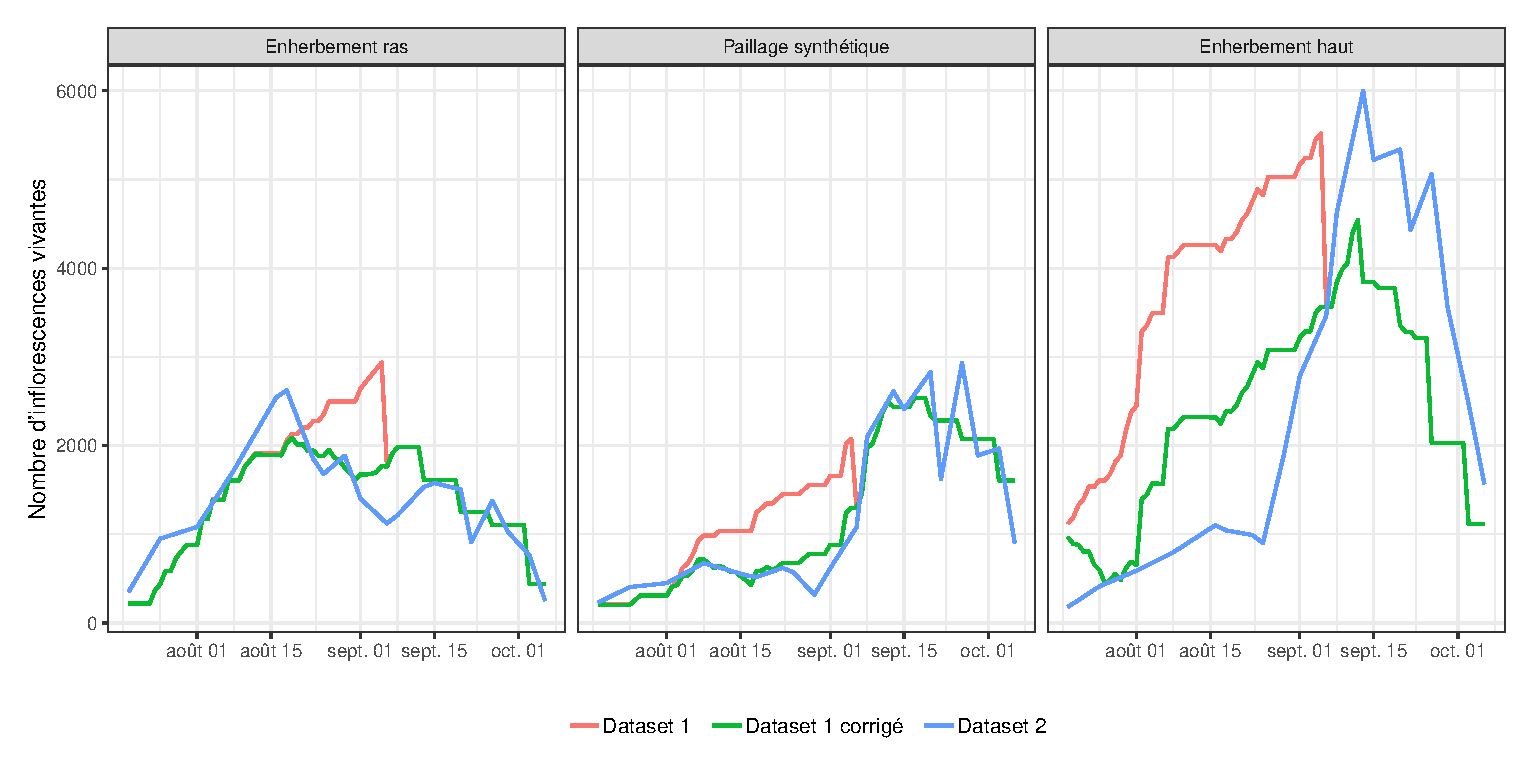
\epsfig{file = r/inflos_vivantes.eps, scale = 0.59}
\caption{Comparaison des différentes dynamiques d'inflorescences vivantes du verger n\textdegree1 en fonction du \emph{dataset} utilisé.}
\label{fig:inflos}
\end{figure}

On fera le choix de privilégier, à chaque fois que cela s'avèrera possible, les dynamiques issues du \emph{dataset 2}.
Ce choix découle du fait que ce sont les dynamiques associées aux dynamiques de larves.


\subsection{Larves}

Le \emph{dataset 2} permet aussi d'extraire la dynamique de larves, à partir des larves piégées.
En effet, on connait le nombre de larves par piège, le nombre d'inflorescences vivantes situées au-dessus des pièges et le nombre d'inflorescences vivantes dans les arbres suivis.
De là, on peut estimer le nombre de larves qui s'éjecte des inflorescences à l'échelle d'un arbre, puis à l'échelle de la sous-parcelle.
Il y a cependant ici une subtilité : le relevé des pièges n'est pas quotidien, il faut donc répartir le nombre de larves piégées entre deux relevés effectifs sur la période entre lesdits relevés.
La dynamiques de larves peut donc s'obtenir en utilisant la formule 
\[
L_t = \frac{N}{n}\left(\sum_{k = 1}^n L_{t}^{k} \times \frac{I_{k, t}^{2}}{I_{k, t}^{2, p}} \right),
\]
où $N$ représente le nombre d'arbre dans la sous-parcelle, $n$ le nombre d'arbre suivis, $I^{2}_{k, t}$ le nombre d'inflorescences sur l'arbre $k$ à la date $t$, $I^{2, p}_{k, t}$ le nombre d'inflorescences au-dessus des pièges dans l'arbre $k$ à la date $t$ et on définit $L_t^k$, le nombre de larves dans les pièges de l’arbre $k$ à la date $t$, par
\[
L_t^k = \frac{L_{k, t}^j}{t^j - t^{j-1}},
\]
avec $t^j$  le nombre de jours entre la première observation et le $j^{\text{ème}}$ relevé et $L_{k, t}^j$ le nombre de larves dans les pièges de l'arbre $k$ au $j^{\text{ème}}$ relevé.
Les différentes dynamiques de larves sont visibles sur la figure~\ref{fig:larves}.
\begin{figure}[ht]
\centering
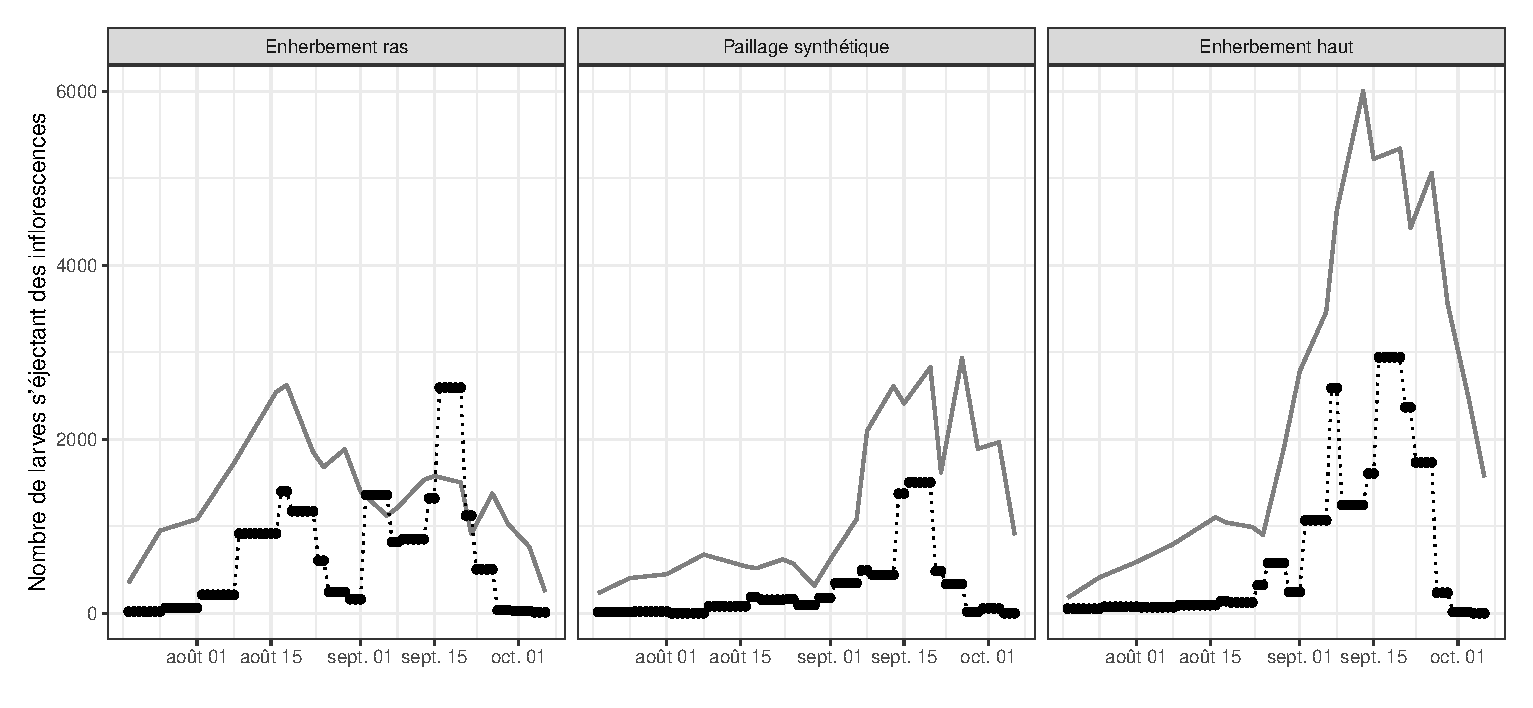
\epsfig{file = r/larves.eps, scale = 0.59}
\caption{Dynamiques de larves s'éjectant des inflorescences des manguiers chaque jour dans le verger n\textdegree1 pour chacune des trois sous-parcelles. En gris sont visibles les dynamiques d'inflorescences vivantes (issues du \emph{dataset 2}, $I^2_t$).}
\label{fig:larves}
\end{figure}

Les dynamiques pour le verger n\textdegree2 sont visibles dans l'annexe~\ref{chap:bloc2}.


% Chapitre 4
\chapter{Le modèle}


\section{Hypothèses}

\section{Formalisme}


% Chapitre 5
\chapter{Calibration du modèle} 

\lettrine{I}{l} est question ici de définir la méthodologie afin de calibrer les paramètres libres du modèle.
On s'intéressera notamment à définir une fonction de coût, pour évaluer la qualité de la calibration.
Dans cette optique, on essayera de calibrer les paramètres en utilisant uniquement les dynamiques du verger n\textdegree1 ; le deuxième servira à la validation.

Il peut être utile de donner la liste des paramètres à calibrer :
\begin{itemize}
 \item $\gamma$, le paramètre relatif à l'arrivée des femelles exogènes ;
 \item $p_{\text{m}}$, le paramètre relatif à la migration des femelles endogènes entre les sous-parcelles ;
 \item $\mu^{1}_{\text{ER}}$ et $\mu^{2}_{\text{ER}}$, les probabilité de réussir à entrer et à sortir du sol pour les cécidomyies pour la modalité «enherbement ras». Pour simplifier,
 on pose $\mu^{1}_{\text{ER}} = \mu^{2}_{\text{ER}}$;
 \item $\mu^{1}_{\text{EH}}$ et $\mu^{2}_{\text{EH}}$, les probabilité de réussir à entrer et à sortir du sol pour les cécidomyies pour la modalité «enherbement haut». Ici aussi,
 on pose $\mu^{1}_{\text{EH}} = \mu^{2}_{\text{EH}}$;
 \item $k$, le paramètre relatif à la disponibilité en ressources pour les inflorescences ;
 \item \texttt{stock}, le nombre de larves entrées en diapause les années précédentes qui décident de sortir l'année considérée ;
 \item $E_0\mu_{\ell}$, le nombre d'œufs pondus par une femelle qui survivent, se transforment en larves puis s'éjectent de l'inflorescences. 
\end{itemize}


\section{Fonction de coût}

Avant une quelconque estimation des paramètres, nous avons besoin de mesurer la qualité de nos estimations.
Pour ce faire, on utilisera une fonction pour comparer le nombre de larves estimées avec le nombre de larves observées. 
Pour définir cette fonction, on pose :
\begin{itemize}
 \item $m$, le nombre de jours entre la première observation et la dernière ;
 \item $n$, le nombre de relevés effectif;
 \item $t$, le nombre de jours passés depuis la première observation ;
 \item $t^j$, le nombre de jours entre la première observation et le $j^{\text{ème}}$ relevé.
\end{itemize}
(On a donc $t^1 = 0$ et $t^n = m$.)

La fonction est alors définie par
$$
f(y, \hat y) = \frac{\sqrt{\frac{1}{n-1}\sum_{j=2}^n\left( y^*_j - \hat y^*_j \right)^2}}{\max(y^*) - \min(y^*)},
$$
où 
$$y^*_j =  y_{t^j} \qquad \text{ et } \qquad \hat y^*_j = \frac{1}{t^j - t^{j-1}}\sum_{k=t^{j-1}}^{t^j} \hat y_k.$$
La figure~\ref{fig:calib} illustre le fonctionnement de la fonction.
Appliquer la fonction à $n-1$ valeurs (correspondant aux relevés sur le terrain) plutôt qu'à chacun des $m$ jours (correspondant à l'étendue des relevés) est motivé par le fait que les relevés ne furent pas fait à des intervalles de temps régulier.
Ce faisant, on évite d'attribuer plus d'importance aux relevés qui ont eu un écart relativement important avec le relevé précédent.

\begin{figure}[ht]
\centering
\begin{tikzpicture}[scale = 0.75]
 \draw [very thin, lightgray, opacity = 0.5] (0,0) grid (13.9, 8.4);
 \draw [->] (0, 0) -- (0, 8.5);
 \draw [->] (0, 0) -- (14, 0);
 \draw (1, 2) node{\textcolor{blue}{$\bullet$}};
 \draw (2, 2) node{\textcolor{blue}{$\bullet$}};
 \draw (3, 2) node{\textcolor{blue}{$\bullet$}};
 \draw (4, 2) node{\textcolor{blue}{$\bullet$}};
 \draw (5, 2) node{\textcolor{blue}{$\bullet$}};
 \draw (6, 2) node{\textcolor{blue}{$\bullet$}};
 \draw (7, 6) node{\textcolor{blue}{$\bullet$}};
 \draw (8, 6) node{\textcolor{blue}{$\bullet$}};
 \draw (9 , 5) node{\textcolor{blue}{$\bullet$}};
 \draw (10, 5) node{\textcolor{blue}{$\bullet$}};
 \draw (11, 5) node{\textcolor{blue}{$\bullet$}};
 \draw (12, 5) node{\textcolor{blue}{$\bullet$}};
 \draw (1, 2.1) node{\textcolor{red}{$\bullet$}};
 \draw (2, 2.9) node{\textcolor{red}{$\bullet$}};
 \draw (3, 3.6) node{\textcolor{red}{$\bullet$}};
 \draw (4, 4.2) node{\textcolor{red}{$\bullet$}};
 \draw (5, 4.6) node{\textcolor{red}{$\bullet$}};
 \draw (6, 4.9) node{\textcolor{red}{$\bullet$}};
 \draw (7, 4.9) node{\textcolor{red}{$\bullet$}};
 \draw (8, 4.7) node{\textcolor{red}{$\bullet$}};
 \draw (9, 4.3) node{\textcolor{red}{$\bullet$}};
 \draw (10, 3.6) node{\textcolor{red}{$\bullet$}};
 \draw (11, 3) node{\textcolor{red}{$\bullet$}};
 \draw (12, 2.2) node{\textcolor{red}{$\bullet$}};
 \draw [dashed] (0.8, 3.716) -- (6.2, 3.716) ;
 \draw [dashed] (6.8, 4.8) -- (8.2, 4.8) ;
 \draw [dashed] (8.8, 3.275) -- (12.2, 3.275) ;
 \draw (0.8, 3.616) -- (0.8, 3.816);
 \draw (6.2, 3.616) -- (6.2, 3.816);
 \draw (6.8, 4.7) -- (6.8, 4.9);
 \draw (8.2, 4.7) -- (8.2, 4.9);
 \draw (8.8, 3.175) -- (8.8, 3.375);
 \draw (12.2, 3.175) -- (12.2, 3.375);
 \draw (3.5, 3.716) node{\textcolor{red}{$\times$}};
 \draw (7.5, 4.8) node{\textcolor{red}{$\times$}}; 
 \draw (10.5, 3.275) node{\textcolor{red}{$\times$}};
 \draw (3.5, 2) node{\textcolor{blue}{$\times$}};
 \draw (7.5, 6) node{\textcolor{blue}{$\times$}}; 
 \draw (10.5, 5) node{\textcolor{blue}{$\times$}}; 
 \draw [<->] (3.5, 2.2) -- (3.5, 3.6);                  
 \draw [<->] (7.5, 5.8) -- (7.5, 5);
 \draw [<->] (10.5, 4.8) -- (10.5, 3.5);
 \draw [fill=white,white] (10.3, 7.01) rectangle (13.9, 8.4);
 \draw (12.2, 8) node {{\small Observation}};
 \draw (12.08, 7.5) node {{\small Estimation}};
 \draw (10.7, 8) node{\textcolor{blue}{$\bullet$}};
 \draw (10.7, 7.5) node{\textcolor{red}{$\bullet$}};
 \draw (6, 0.135) node[rotate = 180] {\textcolor{ForestGreen}{$\intercal$}};
 \draw (8, 0.135) node[rotate = 180] {\textcolor{ForestGreen}{$\intercal$}};
 \draw (12, 0.135) node[rotate = 180] {\textcolor{ForestGreen}{$\intercal$}};
 \draw (7, -0.5) node{\small \text{Temps}};
 \draw  (-0.5, 4.25) node{\rotatebox{90}{\small Larves}};
\end{tikzpicture}
\caption{Schéma illustrant le fonctionnement de la fonction objectif. À chaque relevé effectif (marqueurs verts), on fait correspondre la période correspondant à ce relevé (segments en pointillés).
Et pour chacune de ces périodes, on calcule la moyenne des valeurs estimées (les croix rouges). On compare ensuite les moyennes ainsi calculées avec les valeurs observées associées (les croix bleues).}
\label{fig:calib}
\end{figure}


Par la suite, l'objectif sera de minimiser cette fonction pour chacune des trois sous-parcelles.

\section{Analyse de sensibilité}

Avant de calibrer le modèle, il est pertinent d'effectuer une analyse de sensibilité.
L'analyse de sensibilité est définie par \citet{saltelli2004} comme
\begin{quote}
 «l'étude de comment l'incertitude de la sortie d'un modèle --- qu'elle soit numérique ou non --- peut être répartie entre les différentes sources d'incertitudes présentes dans les entrées du modèle.»\footnote{«The study of how uncertainty in the output of a model (numerical or otherwise) can be apportioned to different sources of uncertainty in the model input.»}
\end{quote}
Autrement dit, on cherche à connaître les paramètres les plus influants sur la sortie du modèle.
La calibration comportant toujours une part d'arbitraire, cette analyse permet de prendre du recul sur les choix de paramètres, relativement à leur impact sur le modèle.
En particulier lorsque certains paramètres ne sont qu'approximatifs vis à vis de la réalité qu'ils ont vocation à décrire, mais fortement significatifs pour la sortie du modèle.

Il existe deux grandes catégories d'analyses de sensibilité, celles qui ont une approche globale et celles qui ont une approche locale (parfois appelées \emph{one-at-the-time}).
L'approche locale consiste à étudier la sensibilité des paramètres les uns après les autres, les uns indépendamment des autres.
Cette approche est valable si et seulement si le modèle est linéaire par rapport à chacune de ses entrées $x_i$ et qu'il n'y a aucune interaction entre les différentes entrées du modèle \citep{saltelli2019so}.
Dès lors qu'il y a la moindre incertitude sur la linéarité du modèle ou sur la non-interaction entre les paramètres, il faut privilégier une approche globale.
Notre modèle n'est pas linéaire et il n'y a dans notre cas aucune raison de supposer la non-interaction entre nos paramètres, bien au contraire.
On utilisera donc une approche globale.

Bien qu'il existe plusieurs méthodes ayant une approche globale, elles ont toutes en commun de fonctionner dans un cadre non-linéaire et de prendre en compte les différentes interactions entre les différents paramètres.
Parmi les méthodes les plus connues et les plus utilisées, on peut en citer qui fonctionnent par décomposition de la variance comme Sobol ou FAST (Fourier Amplitude Sensitivity Test) ou d'autres qui fonctionnent en effectuant des perturbations élémentaires des entrées du modèle comme la méthode Morris.
Notre modèle possède moins de 20 paramètres et s'exécute en moins d'une minute, nous utiliserons alors la méthode Sobol conformément aux recommendations de \citet[chap. 6]{saltelli}.

Le fonctionnement de cette méthode est relativement intuitif.
On considère que la sortie de notre modèle $Y$ peut s'exprimer comme une fonction des entrées de notre modèle $X,$ c'est-à-dire $Y = f(X)$.
Comme $X = \left( X_1, \ldots, X_n \right)$ peut prendre plein de valeurs possibles, il en résulte qu'il y a \emph{a priori} plein de résultats possibles pour $Y.$
% L'objectif est alors de décomposer ces résultats possibles --- cette variance qu'admet $Y$ --- en fonction de chaque entrée du modèle $X_i$.
L'objectif est alors de déterminer quelles entrées du modèle $X_i$ induisent le plus de changements dans ces résultats possibles --- dans cette variance qu'admet $Y.$
À cette fin, on utilise les indices pricipaux de Sobol définis par
\[
S_i = \frac{\textbf{Var}\!\left( \mathbf{E}\!\left[Y|X_i\right] \right)}{\textbf{Var}\!\left( Y \right)}.
\]
% L'indice $S_i$ permet de voir l'effet du seul paramètre $X_i$ sur la variance de $Y$ relativement aux autres.
Ici, $\textbf{Var}\!\left( \mathbf{E}\left[Y|X_i\right] \right)$ permet de voir l'effet du seul paramètre $X_i$ sur la variance de $Y.$
Diviser par la variance totale de $Y$ permet de le faire relativement aux autres paramètres.
Cet indice ne prend cependant pas en compte les interactions entre $X_i$ et les autres entrées du modèle. 
Il faut pour ça utiliser les indices totaux de Sobol définis par
\[
S^T_i = 1 - \frac{\textbf{Var}\!\left( \mathbf{E}\!\left[Y|X_{\sim i}\right] \right)}{\textbf{Var}\!\left( Y \right)},
\]
où $X_{\sim i} = \left(X_1, \ldots, X_{i-1}, X_{i+1}, \ldots, X_n \right)$.
L'indice $S^T_i$ ainsi défini permet lui de prendre en compte l'impact du paramètre $X_i$ et de ses interactions sur la variance de $Y$.
À noter que l'interaction entre $X_i$ et $X_j$ est à la fois prise en compte par $S^T_i$ et $S^T_j$.
C'est pour cette raison qu'il est souvent pertinent d'interpréter les indices principaux et les indices totaux conjointement.

Une fois que l'on connaît la sensibilité du modèle aux différents paramètres, on peut alors passer à la calibration desdits paramètres.


\section{Algorithme d'optimisation}

L'objectif de l'optimisation est de trouver les jeux de paramètres qui minimisent notre fonction de coût, ceux qui permettent d'ajuster au mieux les dynamiques de larves simulées aux dynamiques observées.
Pour ce faire, on a besoin d'un algorithme d'optimisation.
Et il y a du choix.

On peut déjà noter que nous avons sept paramètres à calibrer, et qu'ils évoluent tous dans des intervalles (que l'on définira plus tard).
Il apparaît évident que toutes les solutions ne pourront pas être testées.
Une solution peut être d'utiliser un algorithme basé sur une méthode MCMC comme l'algorithme du recuit simulé.
Nous avons cependant trois dynamiques à ajuster (une pour chaque sous-parcelle), il faudrait alors minimiser la somme (ou la moyenne) des trois fonctions objectifs.
Ou alors on peut directement utiliser un algorithme d'optimisation multicritères.

Ces algorithmes ont l'avantage de pouvoir optimiser simultanément des objectifs qui ne sont pas toujours comparables --- à des échelles différentes, par exemple.
Un des plus connus est sans conteste NSGA-II (Nondominated Sorting Genetic Algorithm II) \citep{deb}.
C'est celui que l'on utilisera.

C'est un algorithme qui ne renvoie pas une unique solution mais un ensemble de solutions. 
Cet ensemble de solutions converge vers un sous-ensemble du front de Pareto.
Le front de Pareto désigne l'ensemble des solutions non-dominées pour un problème donné.
Dans $P \subset \mathbf{R}^{p}$ ($n$ > 1), une solution $x = \left( x_1, \ldots, x_p \right) \in  P$ est dite non-dominée lorsque
\[
\left\{ y \in P\ |\ \forall\ i \in \{1, \ldots, p\},\ y_i \succcurlyeq x_i \text{ et } \exists\ i \text{ tel que } y_i \succ x_i \right\} = \emptyset,
\]
où $\succcurlyeq$ et $\succ$ veulent respectivement dire «au moins aussi bien que» et «meilleur que». 
Dans notre cas, vu que l'on veut minimiser notre fonction de coût, $\succcurlyeq$ se traduira par $\leq$ et $\succ$ se traduira par $<$.
En d'autres termes, $x$ est non-dominée signifie qu'il n'existe pas de solution $y$ qui soit strictement meilleure sur un des critères et au moins aussi bonne sur tous les autres critères.

Le front de Pareto étant un sous-ensemble de $\mathbf{R}^{p}$, il n'est (\emph{a priori}) pas dénombrable.
De ce fait, NSGA-II ne peut pas renvoyer le front tout entier mais seulement un sous-ensemble.
C'est un algorithme itératif, les itérations seront appelées ici \emph{générations}.
Et il faut plusieurs générations pour se retrouver avec des solutions non-dominées.
À la génération $t$, l'algorithme effectue plusieurs opérations.
\begin{enumerate}
 \item On possède un ensemble de solutions potentielles que l'on nommera \emph{population}.
 La taille de la population $N$ est fixée arbitrairement.
 \item À chaque solution de cette population $P_t$, on attribue une solution fille (on verra plus tard comment). 
\end{enumerate}

 Avec la population $P_t$ et les solutions filles associées $F_t$, cela forme un ensemble de solutions potentielles $S_t$ de taille $2N$. 
 On va alors sélectionner parmi ces solutions les $N$ solutions qui nous intéressent le plus.
\begin{enumerate}[resume]
 \item Pour ce faire, pour chaque solution potentielle $s\in S_t$ :
 \begin{itemize}
  \item on calcule le nombre $n_s$ d'éléments de $S_t$ qui domine qui domine $s$ ;
  \item on établit l'ensemble $D_s$ des autres solutions de $S_t$ qui sont dominées par la solution $s$.
 \end{itemize}
 \item On répartit alors nos solutions en plusieurs groupes, en plusieurs \emph{fronts}.
 Vont ainsi dans le premier front $F_1$ les solutions $s$ qui vérifient $n_s = 0$, qui ne sont donc pas dominées par d'autres solutions de $S_t$. 
 Dans le deuxième front $F_2$ se trouvent les solutions qui sont dominées uniquement par les solutions présentes dans $F_1$.
 (Autrement dit, les solutions qui se trouvent dans et uniquement dans $\bigcup_{s\in F_1} D_s$.)
 On continue de la même manière pour $F_3$ (qui contient les solutions uniquement dominées par celles de $F_1$ et $F_2$), $F_4$... jusqu'à ce que toutes les solutions de $S_t$ soient assignées à un front.
 \item On choisira alors de garder en priorité les solutions de $F_1$ puis de $F_2$ et ainsi de suite jusqu'à en obtenir $N$. 
 Il faut noter qu'il existe probablement un front $F_k$ où toutes les solutions ne pourront être garger pour ne pas dépasser la limite imposée de $N$ solutions.
 Plutôt que de choisir aléatoirement le nombre nécésaires de solutions dans $F_k$, seront sélectionnées les solutions qui maximisent une certaine distance --- the \emph{crowding distance} --- avec les autres solutions.
 (On n'entrera pas dans le détail ici.)
 C'est fait pour assurer une certaine diversité entre les différentes solutions.
 Les $N$ solutions ainsi sélectionnées constitueront $P_{t+1}$, la population initiale de la génération suivante $t+1$.
\end{enumerate}

Un élément important pour assurer une convergence vers le front de Pareto est le choix des solutions filles $F_t$ effectué à chaque génération.
Pour générer une solution fille, plusieurs étapes sont là aussi nécessaires.
Ces étapes (simplifiées) sont :
\begin{enumerate}
 \item On selectionne deux solutions $s_1$ et $s_2$ dans $P_t$.
 \item On construit une solution fille $f_1$ en prenant la moitié des coordonnées de $s_1$ et l'autre moitié de $s_2$. 
 On construit $f_2$ en prenant les moitiés de $s_1$ et $s_2$ inutilisées dans la construction de $f_1$.
 \item Sur chacune des solutions filles, une coordonnée choisie aléatoirement est remplacée par une valeur aléatoire choisie dans un intervalle centré sur la valeur initiale.
 \item On réitère ces étapes jusqu'à avoir $N$ solutions filles.
\end{enumerate}


Et c'est ainsi qu'après un nombre suffisant d'itérations, et pour une taille de population suffisament grande, l'algorithme NSGA-II renvoie un ensemble de points suffisament proche du front de Pareto et qui en retranscrit sa diversité.


Dans notre cas, cela signifie que l'on possède différents jeux de paramètres et les valeurs de la fonction de coût pour les trois sous-blocs qu'ils produisent.
Et qu'il ne reste plus qu'à faire un choix.



\section{Exploration de l'ensemble des solutions}


Choisir une solution n'est cependant pas trivial.
En effet, parmi les solutions possibles, aucune n'est objectivement meilleure que les autres.
Il en découle que le choix sera forcément arbitraire.

Plusieurs approches sont possibles.
On peut par exemple choisir au hasard un nombre restreint de solutions possibles, les tester puis sélectionner celle qui semble la plus pertinente.
On peut aussi sélectionner la solution associée aux trois critères qui minimisent une distance à 0, en estimant qu'elle représente un bon compromis entre les différents critères.

Ou alors on essaye d'avoir une vision globale de l'ensemble des solutions.
Il peut même être pertinent de comprendre voire d'\emph{expliquer} quel jeu de paramètres génère quelle solution.
Le choix du jeu de paramètre sera alors plus réfléchi, bien que toujours arbitraire.

Plus précisément, on possède les valeurs de la fonction de coût de nos critères rassemblées dans un tableau $Y$.
On possède également les jeux de paramètres (nos solutions) responsables de ces valeurs rassemblés dans un tableau $X$.
Le but serait alors d'explorer $Y,$ pour savoir par exemple si les critères sont antagonistes (\emph{e.g.} améliorer la prédiction sur une sous-parcelle ne détériore-t-elle pas la prédiction de la sous-parcelle voisine ?) ou alors totalement indépendant.
Mais aussi de pouvoir dire quelles sont les valeurs pour les paramètres $X$ qui minimisent quel critère de $Y$. 
À cette fin, on peut choisir entre deux méthodes : l'ACP-VI  et la régression PLS2.
Nous choisirons la régression PLS2 qui, contrairement à l'ACP-VI, est une méthode régularisante \citep{bry}.
Ce choix nous préserve d'un éventuel problème d'inversibilité de la matrice $X'X$.

On s'intéresse au fonctionnement de la régression PLS2. 
On considère que les tableaux $X$ et $Y$ sont centrés-réduits, $X$ est de dimension $n\times p$, $Y$ est de dimension $n\times q$ et que le rang de $X$ est égal à $a$.
Comme l'explique \citet{tenenhaus}, l'objectif de la régression PLS2 est la «décomposition du tableau $X$ orientée vers l'explication du tableau $Y$».
Si l'on note $\{t_1,\ldots, t_a\},$ une base orthonormée de $X,$ alors il existe des vecteurs $p_h$ tel que l'on puisse écrire
\[
X = \sum_{j = 1}^a t_h p_h'.
\]
Le but est de trouver les composantes $t_h$ qui réalisent un compromis entre deux objectifs. 
Les premières composantes de la base doivent capturer un maximum d'inertie de $X$ en vue d'en réduire la dimension.
Et aussi permettre de prédire au mieux le tableau $Y.$

Le choix de la $h^{\text{ème}}$ composante peut se faire comme suit :
\begin{enumerate}
 \item On s'intéresse à l'information de $X$ qui n'est pas résumée par les $h-1$ premières composantes. 
 Elle est donnée par les résidus de $X$ définis par
 \[
 X^{h-1}_{\cdot j} = X_{\cdot j} - \sum_{\ell=1}^{h-1} p_{\ell j}t_{\ell},  \quad \text{avec } j = 1,\ldots, p.
 \]
 On s'intéresse aussi à l'information de $Y$ qui n'est pas expliquée par les $h-1$ premières composantes de $X$. 
 Cette information est donnée par les résidus de $Y,$
 \[
 Y^{h-1}_{\cdot k} = Y_{\cdot k} - \sum_{\ell=1}^{h-1} c_{\ell k}t_{\ell},  \quad \text{avec } k = 1,\ldots, q.
 \] 
 \item On initiale $u_h$ avec la première colonne de $Y^{h-1}$,
 \[
 u_h = Y^{h-1}_{\cdot 1}.
 \]
 \item On effectue une régression des moindres carrés ordinaires de $X^{h-1}_{\cdot j}$ sur $u_h$ qui passe par l'origine. 
 La pente de cette droite de régression est déterminée par
 \[
 w_{hj} = \frac{X^{h-1'}_{\cdot j} u_h}{u_h'u_h}.
 \]
 On pose $w_h = (w_{h1}, \ldots, w_{hp})'$.
 \item On effectue une régression des moindres carrés ordinaires de $X^{h-1}_{i \cdot} = X_{i\cdot} - \sum_{\ell=1}^{h-1}t_{\ell i}p_{\ell}$ sur $w_h$ qui passe par l'origine. 
 La pente de cette droite de régression est déterminée par
 \[
 t_{hi} = \frac{X^{h-1'}_{i\cdot} w_h}{w_h'w_h}.
 \]
 On pose $t_h = (t_{h1}, \ldots, t_{hn})'$.
 \item On réalise ensuite une régression de $Y^{h-1}_{\cdot k}$ sur $t_h$.
 La pente de la droite de régression des moindres carrés qui passe par l'origine est donnée par
 \[
 c_{hk} = \frac{Y^{h-1'}_{\cdot k} t_k}{t_k't_k}.
 \]
 On pose $c_h = (c_{h1}, \ldots, c_{hq})'$.
 \item On met à jour notre vecteur $u_h$ en effectuant une régression de $Y^{h-1}_{i \cdot} = Y_{i\cdot} - \sum_{\ell=1}^{h-1}t_{\ell i}c_{\ell}$ sur $c_h$.
 La pente de la droite de régression passant par l'origine nous donne 
 \[
 u_{hi} = \frac{Y^{h-1'}_{i \cdot} c_h}{c_h'c_h}.
 \]
 On obtient ainsi notre nouveau vecteur $u_h = (u_{h1}, \ldots, u_{hn})'$.
 \item On réitère les étapes 3 à 6 jusqu'à ce que le vecteur $w_h$ ait convergé.
 \item Enfin, la pente de la droite de régression des moindres carrés de $X^{h-1}_{\cdot j}$ sur $t_h$ qui passe par l'origine nous donne les coefficients $p_{hj}$.
 Ils sont définis par
 \[
 p_{hj} = \frac{X^{h-1'}_{\cdot j} t_h}{t_h't_h}.
 \]
 On en déduit le vecteur $p_h = (p_{h1}, \ldots, p_{hp})'.$
 \end{enumerate}

En plus du formalisme, \citet{tenenhaus} nous donne quelques propriétés sur les différents vecteurs :
\begin{align}
%  t_h't_{\ell} &= 0  &\text{si $\ell \neq h$,} \\
 w_h'p_h &= 1,  \\
%  w_h'X_{\cdot \ell}' &= 0 &\text{pour tout $(h, \ell)$,}\\
 w_h'p_{\ell} &= 0 &\text{si $\ell \neq h$,}\\
 w_h'w_{\ell} &= 0 &\text{si $\ell \neq h$,}\\
%  t_h'X_{\cdot \ell} &= 0 &\text{pour tout $(h, \ell)$,}\\
%  X^{h} &= X\prod_{j=1}^h\left( I - w_jp_j' \right) &\text{pour $h \geq 1$,}\\
 t_h &= X'w_h^* &\text{avec $w_h^* = w_h (p_h'w_h)^{-1}$.} \label{txw}
\end{align}
Ces propriétés s'avèrent utiles pour exprimer $Y$ en fonction des composantes $t_h$, et donc \emph{a fortiori} en fonction de $X$.
Admettons que le nombre de composantes retenues soit $H$.
Par définition des coefficients $c_h$, on peut écrire 
\[
Y = t_1c_1' + \cdots + t_Hc_H' + Y^{H},
\]
où $Y^{H}$ représente les résidus de $Y$, \emph{i.e.} la part de $Y$ qui n'est pas prédite par les composantes $t_1,\ldots,t_H.$
Il peut être utile d'alléger l'écriture en posant $T_H = [t_1 | \cdots | t_H]$. 
On définit $C_H$, $P_H$, $W_H$ et $W_H^*$ de la même manière.
Ainsi,
\begin{align*}
 Y &= T_HC_H' + Y^H\\
 &= XW_H^*C_H' + Y^H & \text{en utilisant la propriété~\ref{txw},}\\
 &= XW_H\left( P_H'W_H \right)^{-1}C_H' + Y^H
\end{align*}
On en déduit $B = W_H\left( P_H'W_H \right)^{-1}C_H'$ correspondant aux coefficients de la régression PLS2 de $Y$ sur $X$ effectué avec $H$ composantes.
Ce qui donne
\begin{align*}
Y_{\cdot k} &\simeq c_{1k}t_1 + \cdots + c_{Hk}t_H\\
&\simeq \left( c_{1k}w_{11}^* + \cdots + c_{Hk}w_{H1}^* \right)X_{\cdot 1} + \cdots + \left( c_{1k}w_{1p}^* + \cdots + c_{Hk}w_{Hp}^* \right)X_{\cdot p}\\
&\simeq b_{k1}X_{\cdot 1} + \cdots + b_{kp}X_{\cdot p}.
\end{align*}
Les variables de $X$ étant centrées-réduites, cela signifie que plus le coefficient $b_{kj}$ sera élevé, plus le paramètre $j$ sera déterminant dans la valeur du critère $k$.












% Chapitre 6
\chapter{Mise en œuvre et résultats} 


\chapter{Discussion} 

\lettrine{O}{n} revient dans ce chapitre sur les résultats obtenus, les hypothèses faites et les méthodes employées.

Commençons par l'aspect biologique.
Bien que l'on ait pas de résultats très pertinents, on peut faire quelques commentaires.
Notamment sur certaines hypothèses qui ont pu être faites.
En premier lieu, le fait que la venue de femelles exogènes se fasse proportionnellement aux inflorescences est une hypothèse forte.
Ce n'est pas très grave dans le cas des solutions--types qui privilégient les individus endogènes, où les femelles exogènes sont peu nombreuses.
Mais cela devient difficile à justifier lorsque les femelles exogènes contribuent fortement aux dynamiques de larves.

Concernant l'hypothèse d'attractivité des inflorescences, ne prendre en compte que les stades phénologiques C, D et E est peut-être un peu radical.
En effet, si le début du stade F commence avec l'apparition de la première fleur cela ne veut pas dire que l'inflorescence devient subitement inattractive pour les cécidomyies.
Si cette attractivité existe bien en réalité, alors ce serait probablement un phénomène plus progressif et le début de la période d'inattractivité interviendrait au milieu du stade F.

La mise en place d'un paramètre de saisonnalité telle que nous l'avons faite est sans doute trop extrême.
Car en pratique, cela revient à éradiquer toutes les femelles (ou les empêcher de pondre) du jour au lendemain, ce qui semble irréaliste.

Bien que l'on ne puisse rien affirmer avec certitude (notamment dû à une absence de validation sur le verger n\textdegree2), ce modèle semble indiquer que quelque chose se produit en fin de saison.
Or, aucune connaissance présente dans la littérature n'explique l'absence de reproduction des cécidomyies autrement que par un changement conséquent de température ou une absence de ressources.
On peut cependant émettre des hypothèses comme, par exemple, une compétition entre la cécidomyie et un autre ravageur qui s'en prendraient aux fleurs des inflorescences et apparaîtraient ainsi qu'à partir du stade phénologique F.

Il faut aussi appuyer sur le fait que la floraison du manguier présente une grande variabilité.
Nous avons pu observer des dynamiques d'inflorescences très différentes au sein d'une même sous-parcelle suite à un échantillonage différent (voir figure~\ref{fig:inflos}).
Il est alors difficile de juger la pertinence du modèle en se basant sur si peu d'observations.
En effet, il suffit que les dynamiques sur lesquelles on calibre le modèle soient atypiques pour que le modèle ne puisse pas se généraliser à d'autres cas.
Difficile de conclure.

On peut également émettre quelques remarques concernant la méthodologie employée.
Concernant l'algorithme d'optimisation, seul NSGA-II a été utilisé.
Et il fonctionne, c'est pourquoi l'on n'en a pas essayé d'autre.
On aurait probablement pu trouver un autre algorithme multicritères qui converge plus vite ou plus près du front de Pareto.
Cependant la diversité des solutions proposées par NSGA-II est déjà grande.
Et avoir des paramètres plus précis n'est peut-être pas pertinent dans la mesure où le phénomène modélisé est très variable et que l'on calibre le modèle sur des données qui ne sont pas elles-mêmes extrêmement précises.

On peut aussi remettre en question la classification effectuée.
Et surtout le choix d'effectuer la classification sur les valeurs de paramètres.
On part ici du principe que deux jeux de valeurs de paramètres dont les valeurs sont proches produiront des dynamiques similaires.
Ce principe ne s'applique pas tous le temps, notamment dans les systèmes chaotiques, où des valeurs initiales très proches peuvent aboutir à des résultats très différents.
Peut-être que dans notre modèle, il se produit --- dans une certaine mesure --- un phénomène similaire, avec notamment la possibilité d'un «effet seuil» chez certains paramètres, qui pourrait produire des dynamiques très différentes malgré des valeurs de paramètres proches.


% Chapitre 7
\chapter{Conclusion} 

\lettrine{S}{i} l'on considère que l'objectif principal du stage était de savoir quelle modalité de couverture du sol et quelle dynamique d'inflorescences permettent de limiter l'impact de la cécidomyie des fleurs sur un verger de manguiers, alors le stage est un échec.
Il faut néanmoins relativiser. Il y avait plusieurs objectifs au stage.

Le premier était de modéliser le système manguier -- cécidomyies des fleurs.
Le modèle existe et il est fonctionnel.
Cet objectif est atteint.

Le deuxième objectif était d'analyser le fonctionnement dudit système.
Bien que nous n'avons pas été capable de proposer une solution reproduisant les observations effectuées sur le terrain, cet objectif est partiellement rempli.
En effet, le modèle semble mettre en évidence l'existence d'un phénomène en fin de saison responsable de la diminution du nombre de cécidomyies, ce qui permet 
d'envisager de nouvelles pistes pour mieux comprendre le système.

Le troisième objectif était de réaliser des tests \emph{in silico} afin d'évaluer le meilleur mode de gestion des vergers.
Cet objectif n'a en revanche pas été atteint.

À l'issue de ce stage, on peut envisager plusieurs pistes pour de futures tentatives.
Par exemple, réaliser de nouvelles expérimentations sur le terrain pour acquérir plus de données.
Et aussi s'intéresser à la possible compétition entre la cécidomyie des fleurs et d'autres ravageurs.
Il faudra \emph{a priori} avoir plus de connaissances et/ou de données avant d'entreprendre à nouveau une démarche de modélisation.

\paragraph{ } D'un point de vue personnel, ce stage aura été une réussite.
D'abord d'un point de vue technique. J'ai pu appliquer des concepts mathématiques appris en cours à un cas concret.
J'ai aussi été amené à apprendre par moi-même non vus en cours, et à les appliquer. Cela fut très intéressant.

Ensuite d'un point de vue professionnel, j'ai pu avoir une première expérience dans le domaine de la recherche.
Expérience fort plaisante, qui m'a permis de me faire une idée plus précise du métier de chercheur.
Et de rappeler certaines évidences : les résultats obtenus ne sont pas toujours présents ou ne sont pas toujours ceux que l'on cherche initialement, et que cette incertitude est au cœur même du métier.


% Remerciements obligatoires
\section*{Remerciements}

Ce rapport de stage a été réalisé dans le cadre du projet ECOVERGER, action pilotée par le ministère de l’Agriculture et de l’alimentation et le ministère de la Transition écologique et solidaire, avec l’appui financier de l’Agence française pour la biodiversité dans le cadre de l'APR «Résistance et pesticides» grâce aux crédits issus de la redevance pour pollutions diffuses attribués au financement du plan Ecophyto et dans le cadre du programme de recherche agronomique du Cirad à la Réunion, DPP COSAQ, financé par la communauté européenne (fond structurel FEDER) et le Conseil Régional de La Réunion.





\begin{figure}[!h]
 \centering
 \includegraphics[scale = 0.3]{photos/ecoverger.png}
\end{figure}



\begin{figure}[!h]
 \centering
 \includegraphics[scale = 0.3]{photos/cosaq.png}
\end{figure}


\bibliography{biblio}

\appendix

% Graphiques verger 2
 \chapter{Verger n\textdegree2}
 \label{chap:bloc2}
 
 On présente ici le dispositif présent sur le verger expérimental n\textdegree2 ainsi que les dynamiques d'inflorescences et de larves obtenues grâce aux données des relevés effectués sur cette parcelle.
 
 Le dispositif mis en place était similaire à celui du verger n\textdegree1, à la différence de l'ordre des modalités de couverture du sol (voir figure~\ref{fig:schema2}).
 
 \begin{figure}[ht]
 \centering
 
 \begin{tikzpicture}[scale = 0.4]
  \draw (0,5) rectangle (18, 12);
  \draw (6, 5) -- (6, 12);
  \draw (12, 5) -- (12, 12);
  \draw (-0.5, 0) -- (-0.5, 3) ;
  \draw (-0.5, 3) -- (18.5, 3) ;
  \draw (18.5, 3) -- (18.5, 0);
  \draw (9, 1.75) node{\text{ \footnotesize Autre verger de manguiers}};
  \draw (9, 0.75) node{\text{\footnotesize (possible source d'infestation)}};
  \draw (9, 9) node{\text{ \footnotesize Enherbement}};
  \draw (9, 8) node{\text{ \footnotesize haut}};
  \draw (3, 9) node{\text{ \footnotesize Enherbement}};
  \draw (3, 8) node{\text{ \footnotesize ras}};
  \draw (15, 9) node{\text{ \footnotesize Paillage}};
  \draw (15, 8) node{\text{ \footnotesize synthétique}};
  \draw (-0.5, 4.5) rectangle (18.5, 14);
  \draw (9, 13) node{\text{ \footnotesize Verger expérimental }};
 \end{tikzpicture}
 \caption{Schéma de l'expérimentation menée. Le verger sur lequel ont été testées les trois modalités de couvertures du sol était situé à côté d'un autre verger. Bien que cet autre verger n'avait pas de rôle particulier, il a probablement servi de source d'infestation exogène au verger expérimental.}
 \label{fig:schema2}
\end{figure}
 
 Le verger n\textdegree2 présente des caractéristiques particulières, rajoutant des différences supplémentaires entre les différentes sous-parcelles, en plus des différentes modalités.
 Ce verger est disposée «en escalier», avec une modalité sur chaque «marche».
 L'ensoleillement n'était pas le même entre les différentes modalités, et cela se ressent sur la figure~\ref{fig:inflos2}.
 La sous-parcelle avec un paillage synthétique --- la plus ensoleillé --- présente ainsi plus d'inflorescences que les deux autres.
 On retrouve aussi des différences d'inflorescences entre les parcelles enherbées, celle avec l'enherbement haut avait plus de soleil que l'autre, et elle a eu plus d'inflorescences.
 
 \begin{figure}[ht]
\centering
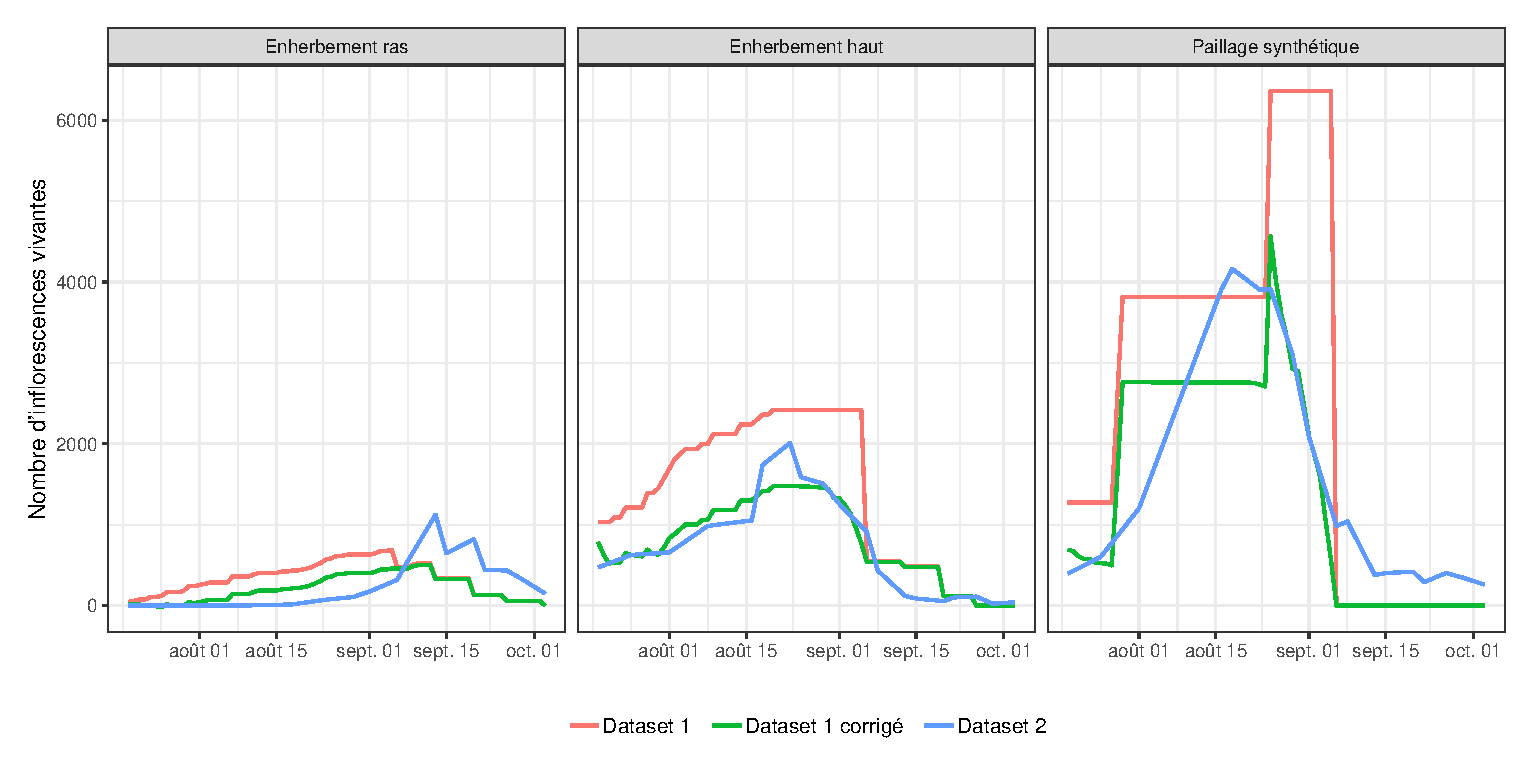
\epsfig{file = r/inflos2.eps, scale = 0.59}
\caption{Comparaison des différentes dynamiques d'inflorescences vivantes du verger n\textdegree2 en fonction du \emph{dataset} utilisé. Même après correction, on observe des différences entre les dynamiques issues des différents jeu de données, en particulier pour les deux premières modalités.}
\label{fig:inflos2}
\end{figure}
\newpage
 On peut noter aussi des différences entre les deux jeux de données. C'est flagrant pour la modalité «paillage synthétique», où il n'y a seulement que 5 observations dans le \emph{dataset 1} produisant cette dynamique particulière. À cela se rajoute la variabilité du phénomène donnant des dynamiques très différentes pour des échantillonnages différents. Seule la sous-parcelle avec un enherbement haut présente des dynamiques similaires entre les deux jeux de données.
 
 Les dynamiques de larves pour ce verger sont visibles sur la figure~\ref{fig:larves2}.
 
 \begin{figure}[ht]
\centering
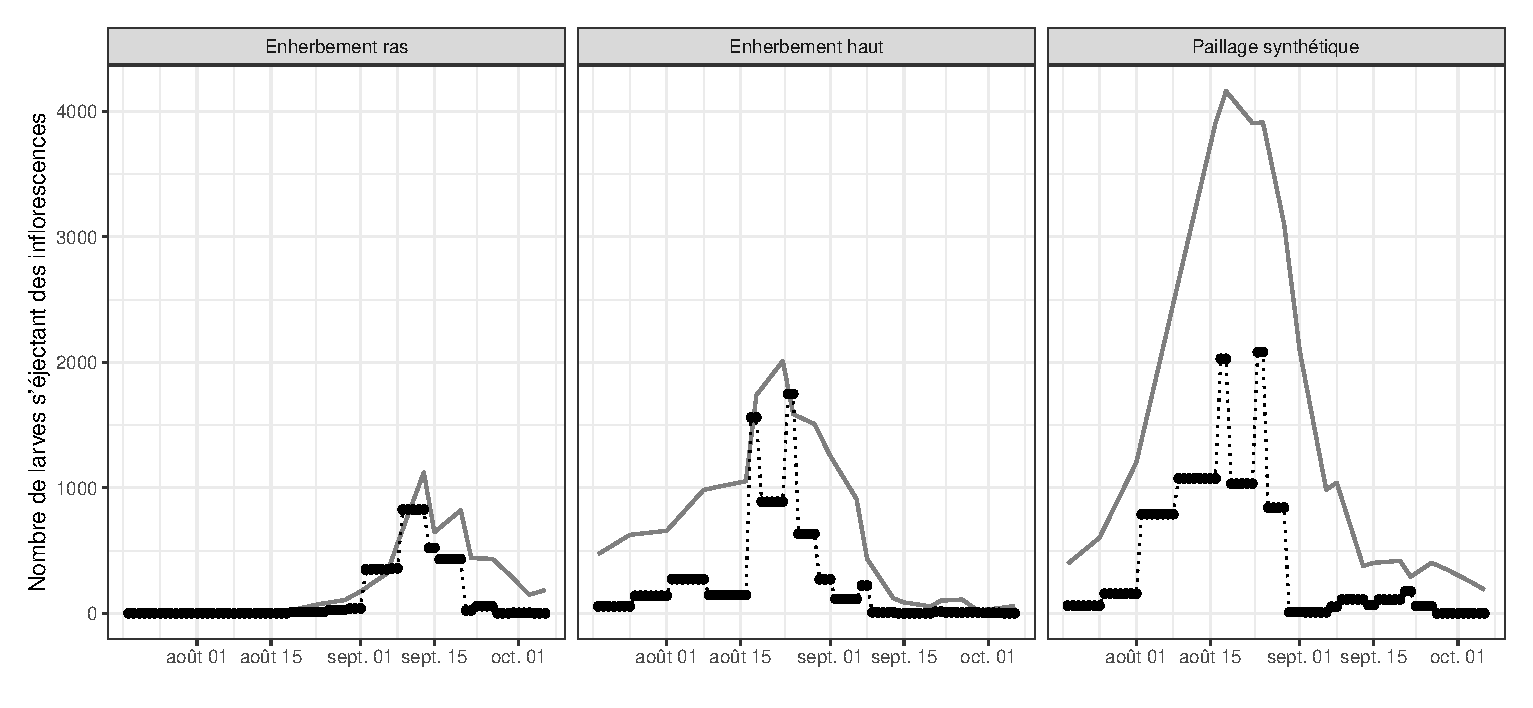
\epsfig{file = r/larves2.eps, scale = 0.59}
\caption{Dynamiques de larves s'éjectant des inflorescences des manguiers chaque jour dans le verger n\textdegree2 pour chacune des trois sous-parcelles. En gris sont visibles les dynamiques d'inflorescences vivantes (issues du \emph{dataset 2}, $I^2_t$).}
\label{fig:larves2}
\end{figure}



% Pupaison
% \chapter{Expression de la pupaison en fonction de la température}
\label{chap:pupaison}

Jusqu'à présent nous avions dans notre modèle $p_{\text{p}}$ fixé à 0.77. 
En utilisant une constante, on ne prend pas du tout en compte les conditions externes qui pourrait influencer sur le cycle de développement des cécidomyies (\emph{e.g.} les conditions météorologiques).
 
Le but est ici d'obtenir une valeur de $p_{\text{pup}}$ qui dépendrait de la température. On choisit la température car cette variable est accesible et qu'elle a, \emph{a minima}, un effet sur la durée de la diapause \citep{pauldiap}.

On récupère les données de l'article de \citet{pauldiap} pour essayer de voir s'il y a un lien entre température et durée de pupaison.

À chaque date --- pour lesquelles on a des données sur le nombre de larves et le nombre de larves en pupaison --- on calcule la proportion de larves en pupaison.
On extrait ensuite les températures moyennes sur 15 jours (de 7 jours avant jusqu'à 7 jours après) pour chaque jour où l'on a des données disponibles.
Le choix de prendre la température moyenne sur 15 jours est fait pour prendre au mieux en compte les conditions climatiques qu'il y a eu avant l'enfouissement (et notamment au moment de la ponte) et après l'enfouissement (durant la pépriode de pupaison).
On effectue une régression linéaire simple de la proportion de larves en pupaison par la température.

On fixera le seuil du risque de première espèce à $\alpha = 5\%$ pour le test de non-nullité des coefficients.
Les résultats sont visibles dans la table~\ref{tab:lm2}.
On en conclut que les coefficients associés à l'ordonnée à l'origine et à la température ne sont pas nuls et que l'on peut écrire
\[
p_{\text{p}} = 1.9555 - 0.055\times t_{15j}.
\]

\begin{table}[hb]
\centering
\caption{Régression linéaire simple de la proportion d'individus en pupaison par la température moyenne sur 15 jours}
\label{tab:lm2}
\begin{tabular}{rrrrr}
 & Estimate & Std. Error & t value & Pr($>$$|$t$|$) \\ 
  \hline
(Intercept) & 1.9555 & 0.3665 & 5.34 & 0.0002 \\ 
  temp15j & -0.0550 & 0.0160 & -3.43 & 0.0050 \\ 
\end{tabular}
\end{table}


% Débourrements
\chapter{Simulation d'inflorescences attractives} 
\label{chap:deb}

On détaille dans cette annexe comment simuler des dynamiques d'inflorescences attractives.
Pour ce faire, nous avons besoin des dates de débourrements des inflorescences ainsi que de la loi de mortalité des inflorescences.


Le \emph{dataset 1} contient des dates de débourrements. On ne pourra cependant pas les utiliser.
Dans le verger n\textdegree1, les dynamiques pour les modalités «enherbement ras» et «paillage synthétique» issues des deux jeux de données ont des dynamiques plutôt similaires ; on pourrait donc utiliser les débourrements du \emph{dataset 1} mis à l'échelle.
En revanche, pour la modalité «enherbement haut», on observe des dynamiques très différentes. 
Et comme l'on souhaite privilégier les dynamiques issues du \emph{dataset 2} (qui sont associées aux dynamiques de larves), il faut procéder autrement.
(Il en va de même pour les modalités «enherbement ras» et «paillage synthétique» du verger n\textdegree2.)
 
L'objectif est alors de simuler les dates de débourrements qui permettent de produire la dynamique d'inflorescences vivantes du \emph{dataset 2}.
Pour cela, on suppose que la durée de vie effective d'une inflorescence suit une loi normale.
On possède les durées de vies effectives dans le \emph{dataset 1}.
Premièrement, en fixant le risque de première espèce à $\alpha = 5\%$, un test de normalité de Shapiro--Wilk nous confirme la normalité ($p$-valeur de 0.05447, on ne rejette donc pas l'hypothèse de normalité).
Deuxièmement, on observe une durée de vie effective moyenne de 29 jours (avec un écart-type de 14).
Ainsi, il faut donc simuler des débourrements, pour que des inflorescences ayant une durée de vie qui suit une $\mathcal{N}\left( 29; 14 \right)$, donne la dynamique d'inflorescences vivantes du \emph{dataset 2}.
Il faut donc trouver les $B_t$ tels que 
\[
I_{t}^{2} = B_t + \sum_{j = 1}^{50} B_{t - j} \times \left( 1 - F\left( j \right) \right),  \qquad \text{ avec } B_{t} = 0 \text{ si } t \leq 0,
\]
où $F$ est la fonction de répartition d'une $\mathcal{N}\left( 29;14 \right)$ et 50 la durée de vie théorique d'une inflorescence.
 
Par souci d'homogénéité, on utilisera les débourrements simulés pour les trois modalités, et ce pour les deux vergers.



Les inflorescences \emph{attractives} peuvent alors se calculer en utilisant la formule
\[
I_{t}^{a} = B_t + \sum_{t = 1}^{d_A} B_{t-j} \times \left( 1 - F(j) \right), \qquad \text{ avec } B_{t} = 0 \text{ si } t \leq 0. 
\]
Ici, $B_t$ représente le nombre de débourrements à la date $t$, $d_A$ la durée d'attractivité voulue et $F$ la fonction de répartition d'une $\mathcal{N}\left( 29; 14 \right)$.

Dans notre cas, on choisira $d_A = 16$ jours, correspondant à la durée des stades C, D et E.


% Pupaison chelou
\chapter{Calibration de la probabilité d'entrer en phase de pupaison} 
\label{chap:pup_chelou}

On s'intéresse ici à une version du modèle qui diffère légèrement de celle décrite dans la partie~\ref{chap:temp}.
On cherche toujours à ajuster la probabilité d'entrer en phase de pupaison en fonction de la température.

On repart de la formule
\[
p_{\text{p}} = 1.9555 - 0.055\times t_{15j},
\]
à laquelle on rajoute la possibilité d'effectuer certaines modifications.
On introduit deux coefficients, $\varpi\in [1; 4]$ et $p_{\text{p}}^*\in [0; 1]$, comme suit :
\[
\widetilde p_{\text{p}} = \left( p_{\text{p}} - \overline{p_{\text{p}}} \right) \times \varpi + p_{\text{p}}^*,
\]
où $\widetilde p_{\text{p}}$ sera la probabilité d'entrer en pupaison et d'y survivre utilisée par le modèle et $\overline{p_{\text{p}}}$ la moyenne de la probabilité de pupaison.
Comme dans la partie \ref{chap:temp}, le coefficient $\varpi$ permet au modèle d'amplifier la variabilité de la probabilité d'entrer en pupaison.
La nouveauté est ici le coefficient $p_{\text{p}}^*$, qui permet au modèle de calibrer la probabilité d'entrer en pupaison moyenne sur la saison.





La figure~\ref{fig:params} montre les valeurs trouvés après calibration pour les deux paramètres présentés ci-dessus.
Et il s'avère qu'il n'y a  que très peu de variabilité pour les deux paramètres, les deux étant très souvant fixés à 1.




\begin{figure}
 \centering
 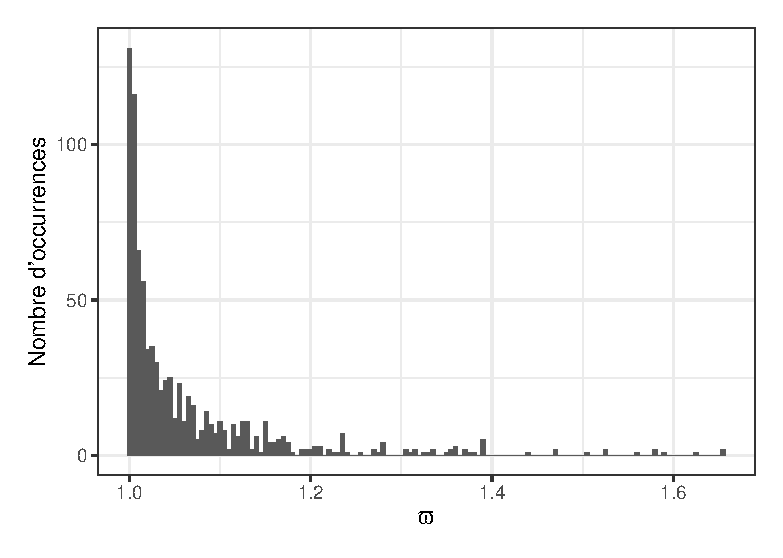
\epsfig{file = plots/varpi.eps, scale = 0.55}
 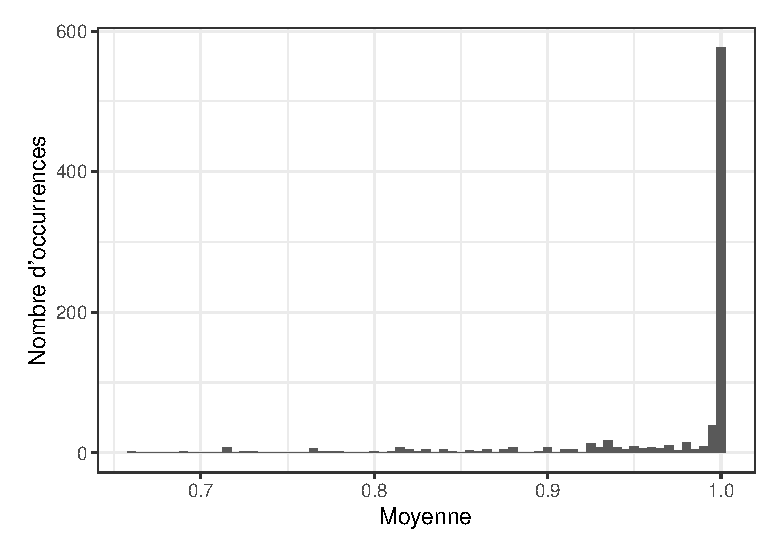
\epsfig{file = plots/intercept.eps, scale = 0.55}
 \caption{Résultats de la calibration pour les paramètres $\varpi$ et $p_{\text{p}}^*$.}
 \label{fig:params}
\end{figure}


Or, comme le montre la figure~\ref{fig:prob}, il en résulte que la probabilité d'entrer en pupaison est quasi-constante.
La seule différence avec le modèle initial est que cette quasi-constante est proche de 1 au lieu de 0.77.

\begin{figure}
 \centering
 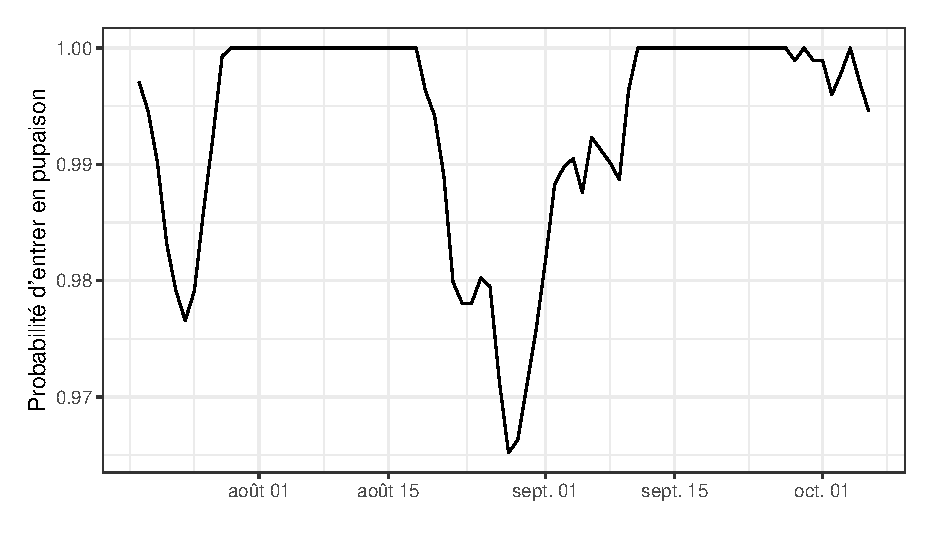
\epsfig{file = plots/pupaison_chelou.eps, scale = 0.7}
 \caption{Probabilité d'entrer en phase de pupaison obtenue lorsque $\varpi = 1$ et $p_{\text{p}}^* = 1$.}
 \label{fig:prob}
\end{figure}

On retrouve, sans surprises, trois solutions--type qui sont très similaires à celles des parties~6.1 et \ref{chap:temp}.
Il apparaît alors peu utile de les afficher.


% Durée attractivité
\chapter{Calibration de la durée d'attractivité} 
\label{chap:attra}

On s'intéresse ici aux résultats produits par le modèle décrit dans la section~\ref{chap:cde}, à la différence que le modèle calibre aussi la durée d'attractivité $d_A$.
On laisse au modèle la possibilité d'avoir une durée d'attractivité $d_A$ comprise entre 3 et 40 jours.

La figure~\ref{fig:da} montre la fréquence des différentes durées d'attractivité obtenues après la calibration du modèle.
Il y a trois durées d'attractivité qui le modèle semble privilégier : 3 jours, 11 jours et 40 jours.
On notera cependant que les durées égales à 3 jours et 40 jours correspondent aux bornes définies pour la calibration.
Une durée d'attractivité égale à 3 jours semble peu réaliste, une durée d'attractivité de 40 jours ne donne pas des dynamiques d'inflorescences significativement différentes avec les dynamiques d'inflorescences vivantes.
On ne s'intéressera donc qu'aux résultats dont la durée d'attractivité est comprise entre 9 et 16 jours.

\begin{figure}[ht]
 \centering
 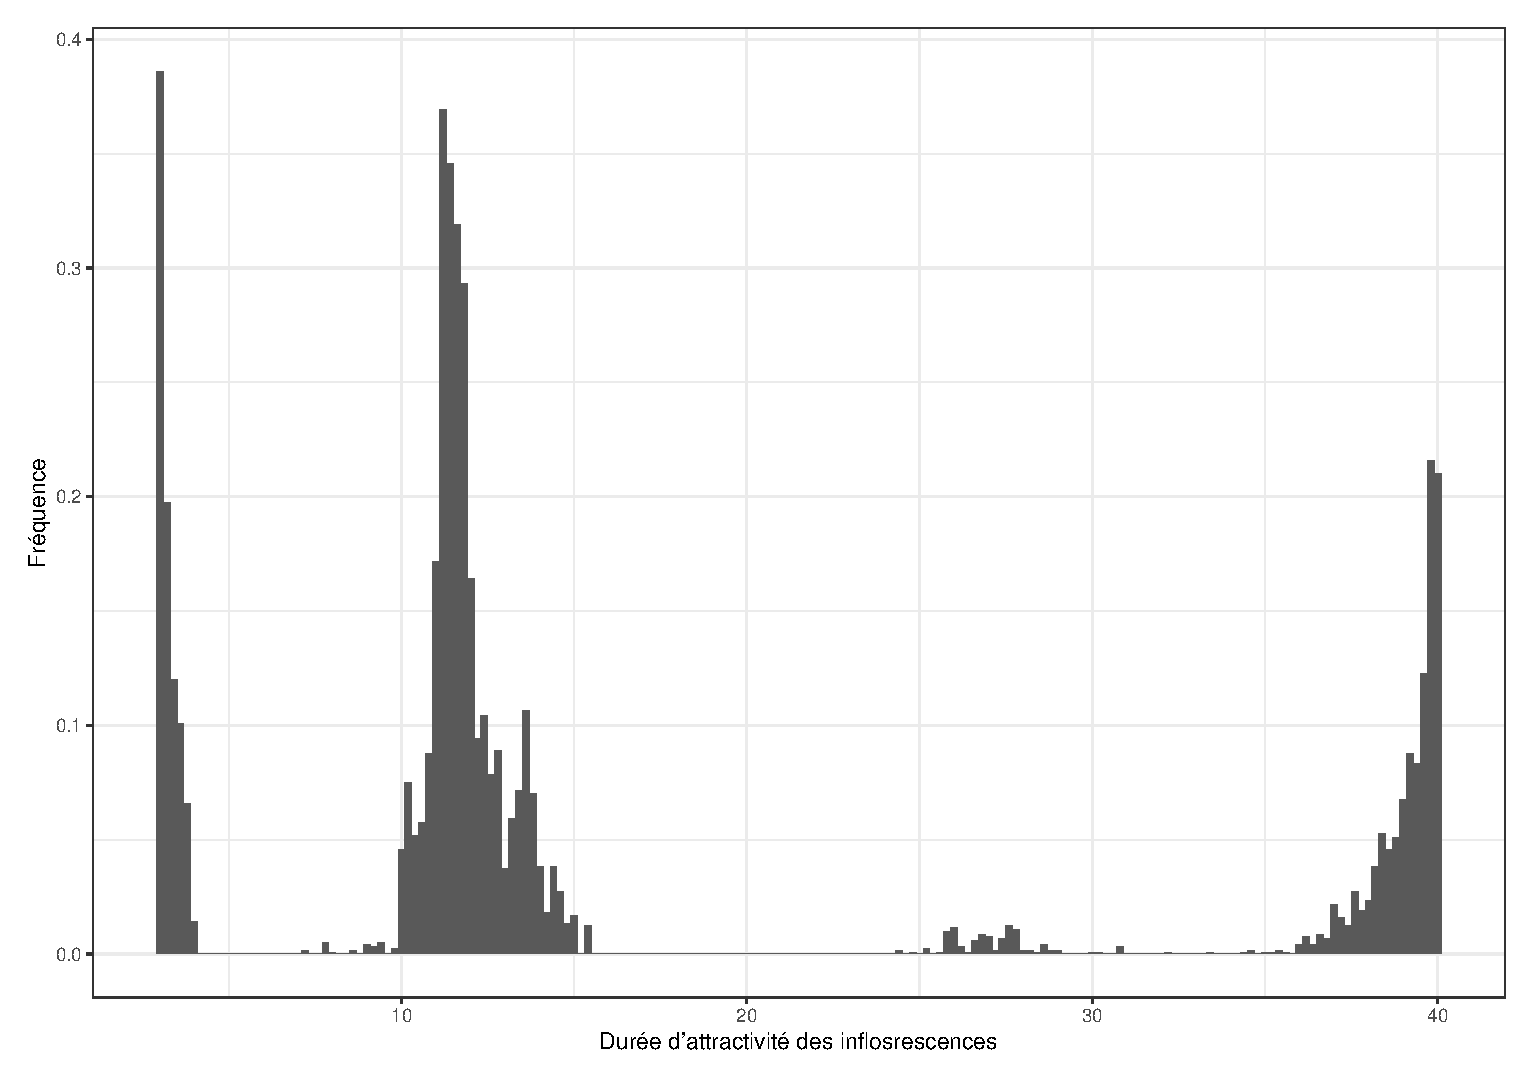
\epsfig{file = plots/dA.eps, scale = 0.43}
 \caption{Fréquence des durées d'attractivité calibrées}
 \label{fig:da}
\end{figure}

Il y a 641 solutions non-dominées dont la durée d'attractivité est comprise entre 9 et 16 jours.
Après classification des solutions, trois solutions types se dégage :
\begin{itemize}
 \item \textbf{Solution--type 1 :} La première solution--type contient beaucoup d'individus exogènes, peu d'échanges entre les trois sous-parcelles, et peu d'individus émergeant de la sous-parcelle EH.
 Il en résulte que, sur les sous-parcelles PS et EH, la population de femelles est essentiellement exogènes. Ce qui paraît peu réaliste.
 En outre, les dynamiques de larves ne sont pas très bien captées.

 Les paramètres associées à cette solution sont :
 \begin{center}
\begin{tabular}{llllllll}
$\gamma$ & $p_{\text{m}}$ & $\mu_{\text{ER}}$ & $\mu_{\text{EH}}$ & $k$ & \texttt{stock} & $E_0\mu_\ell$ & $d_A$\\
0.059 & 0.042 & 0.533 & 0.116 & 1.928 & 500 & 7.517 & 10.3
 \end{tabular}
 \end{center}

 \item \textbf{Solution--type 2 :} Il y a dans la deuxième solution--type des échanges entre les sous-parcelles, cela conduit à des dynamiques de larves assez bien captées sur les sous-parcelles PS et EH.
 En revanche, le niveau d'individus exogènes reste élevé et la dynamique de la sous-parcelle ER toujours aussi mal captée.
 
 Les paramètres produisant cette solution sont :
  \begin{center}
\begin{tabular}{llllllll}
$\gamma$ & $p_{\text{m}}$ & $\mu_{\text{ER}}$ & $\mu_{\text{EH}}$ & $k$ & \texttt{stock} & $E_0\mu_\ell$ & $d_A$\\
0.047 & 0.389 & 0.832 & 0.036 & 1.347 & 522 & 6.466 & 11.5
 \end{tabular}
 \end{center}
 
 \item \textbf{Solution--type 3 :} À la différence des deux autres solutions, il y a peu d'individus exogènes. On note également que les dynamiques de larves captées dans les sous-parcelles PS et EH sont tout à fait satisfaisantes.
 On peut cependant déplorer la mauvaise prédiction sur la sous-parcelle ER.
 
 Les paramètres associées sont :
   \begin{center}
\begin{tabular}{llllllll}
$\gamma$ & $p_{\text{m}}$ & $\mu_{\text{ER}}$ & $\mu_{\text{EH}}$ & $k$ & \texttt{stock} & $E_0\mu_\ell$ & $d_A$\\
0.014 & 0.284 & 0.813 & 0.018 & 0.220 & 6523 & 8.403 & 13.8
 \end{tabular}
 \end{center}
 
\end{itemize}

Les dynamiques sont visibles dans la solution~\ref{fig:C2}.

On notera aussi qu'il n'y a aucune solution avec des individus émergeant de la sous-parcelle EH.


\begin{figure}[ht]
 \centering
 \textbf{Solution--type 1}
 
 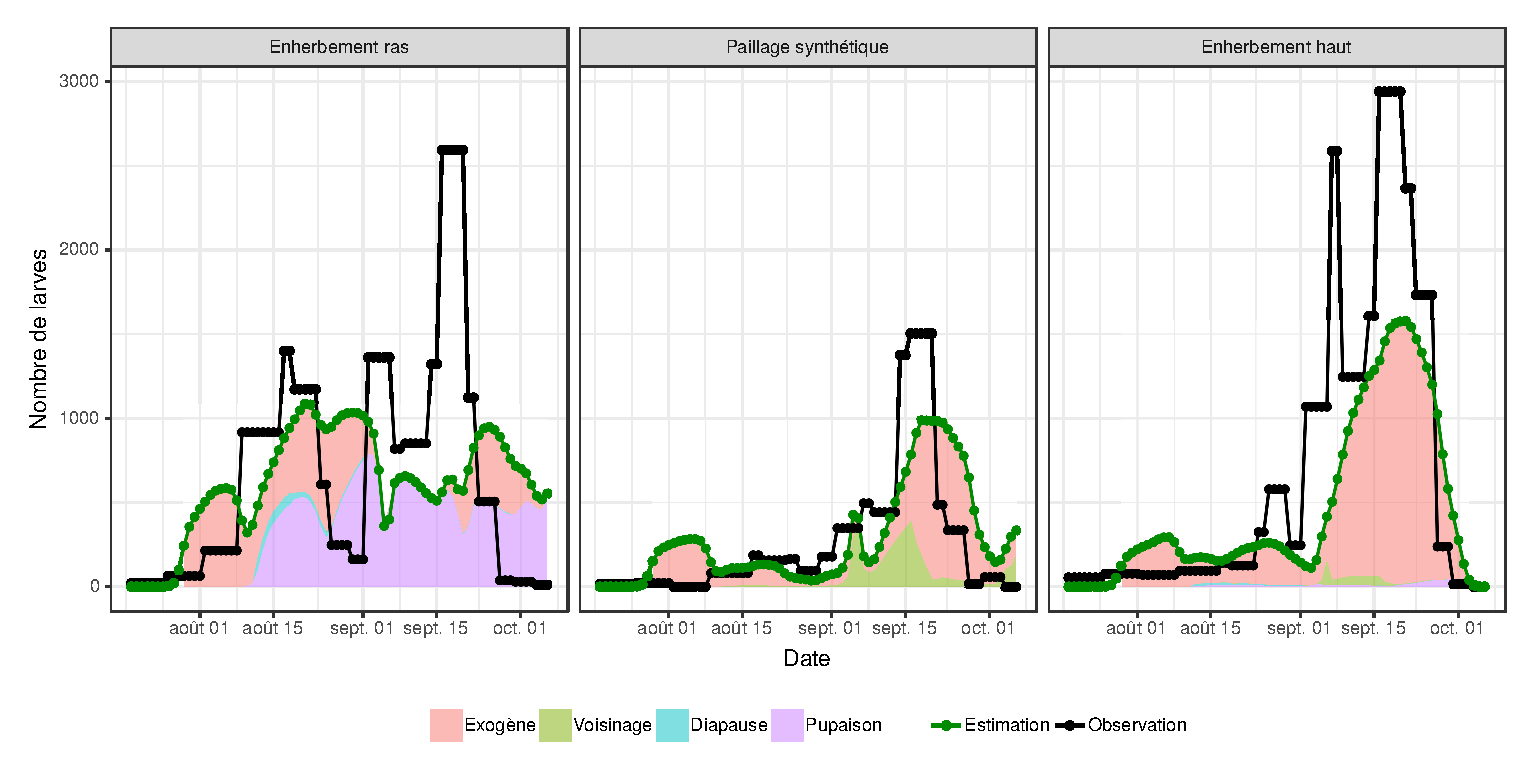
\epsfig{file = plots/C2_1.eps, scale = 0.52}
 
 \textbf{Solution--type 2}
 
 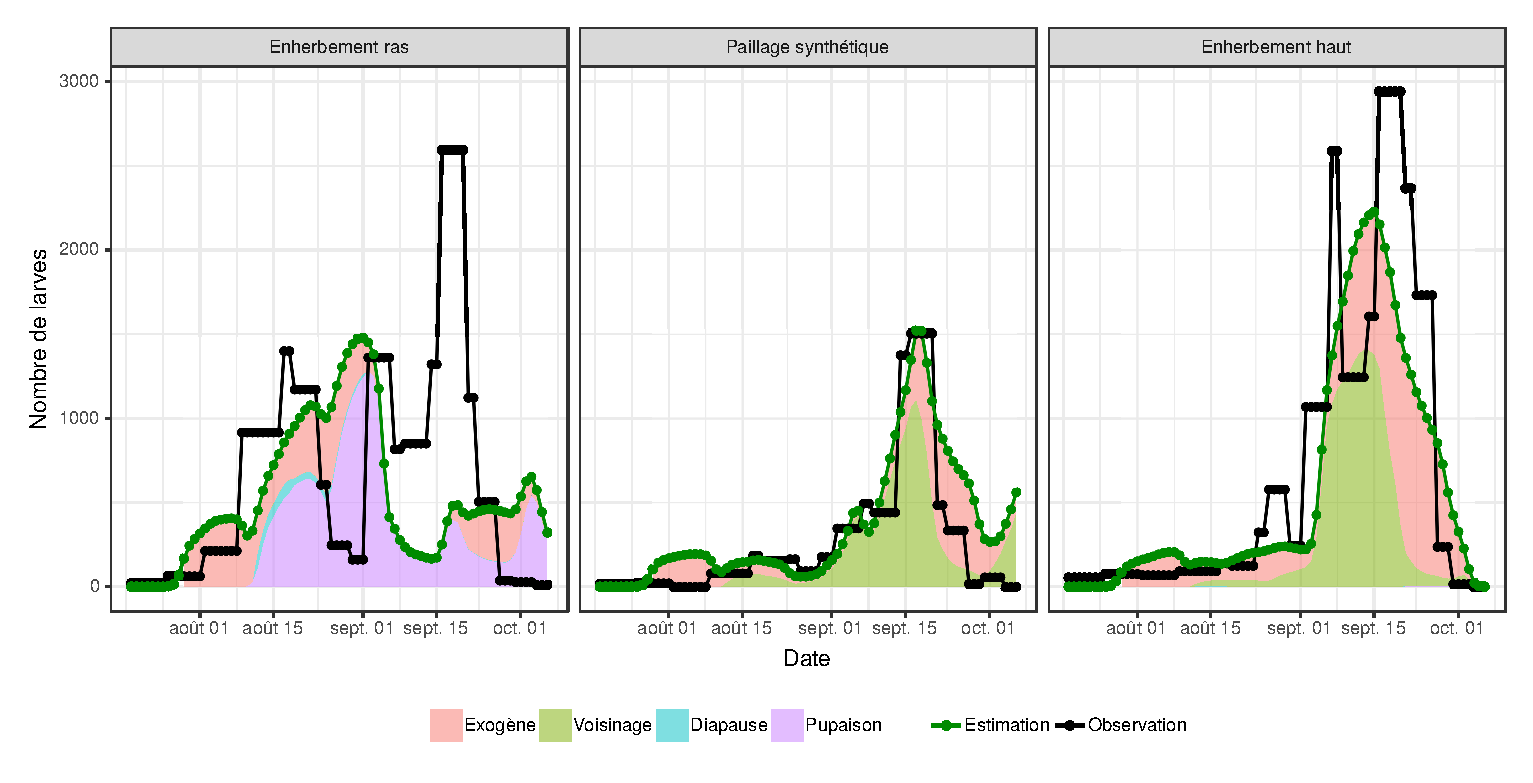
\epsfig{file = plots/C2_2.eps, scale = 0.52}
 
 \textbf{Solution--type 3}
 
 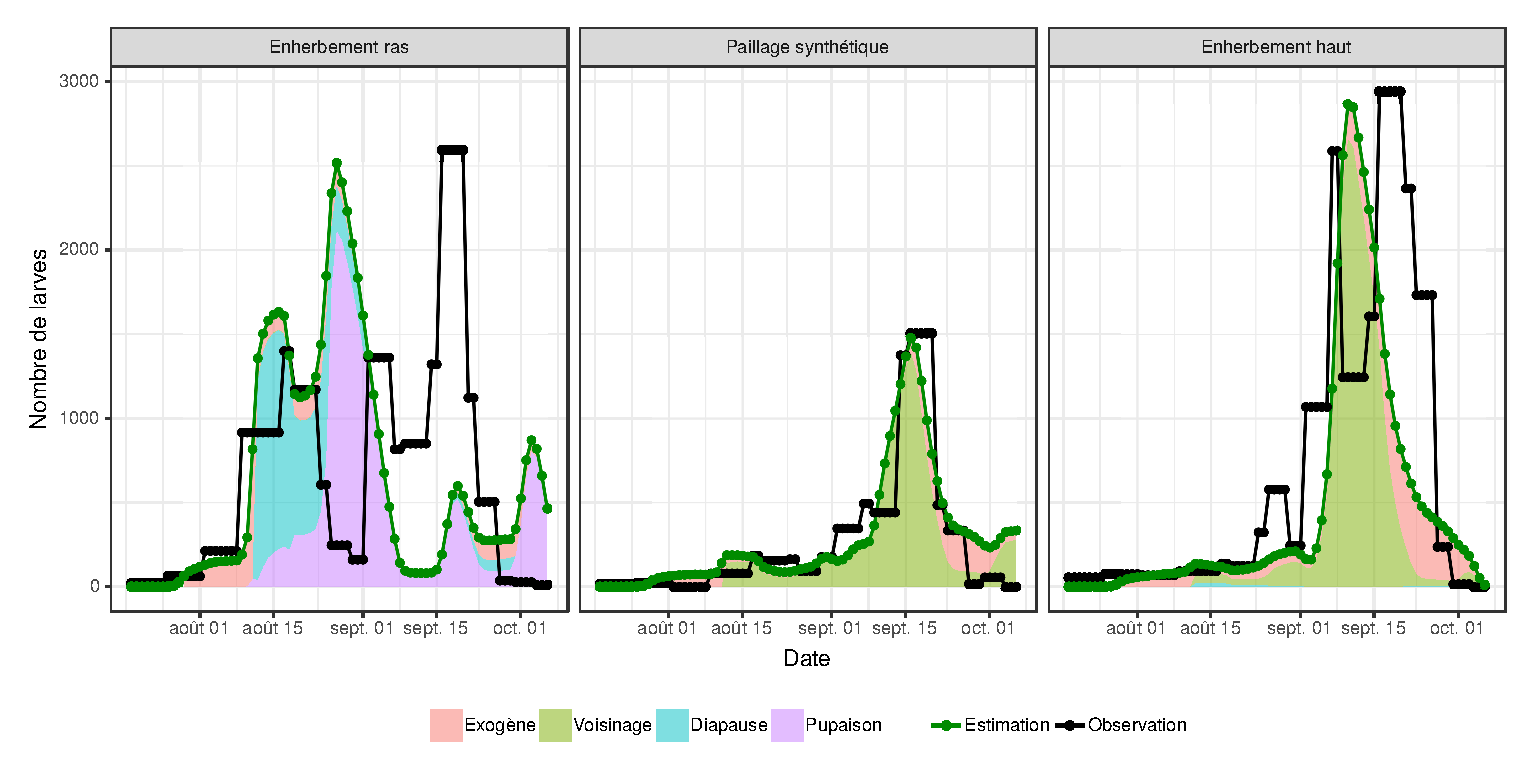
\epsfig{file = plots/C2_3.eps, scale = 0.52}
 \caption{Dynamiques observées et simulées pour chacune des trois solutions--types. La décomposition indiquant la provenance des femelles qui ont pondus les œufs est disponible pour les dynamiques simulées.}
 \label{fig:C2}
\end{figure}


% Durée développement
\chapter{Calibration de la durée de développement larvaire} 

Dans les différents modèles testés, les larves s’éjectent entre 7 et 12 jours après la ponte.
La répartition de la sortie des larves est la suivante :
\begin{center}
\small
\begin{tabular}{lllllll}
\textbf{Nombre de jour après la ponte} & Jour 7 & Jour 8 & Jour 9 & Jour 10 & Jour 11 & Jour 12\\
\textbf{Proportion} & 0.025 & 0.075 & 0.4 & 0.4 & 0.075 & 0.025
\end{tabular}
\end{center}

Dans cette annexe, on s'intéresse au cas où le modèle calibre aussi la durée de développement larvaire.
On ne modifiera cependant ni l'étendue d'éjection des larves vers le sol (6 jours) ni la distribution de sortie des larves.
En pratique, le modèle calibrera uniquement le premier jour d'éjection des larves vers le sol, entre 1 et 10.

Par ailleurs, on utilisera en entrée du modèle les inflorescences aux stades phénologiques C, D et E. Et la probabilité  d'entrer en pupaison pour les larves dépendra linéairement de la température.

Après calibration du modèle, on s'intéresse au premier jour d'enfouissement après la ponte que renvoie le modèle. Les résultats sont visibles sur la figure~\ref{fig:duree_dvpmt}.

\begin{figure}
 \centering
 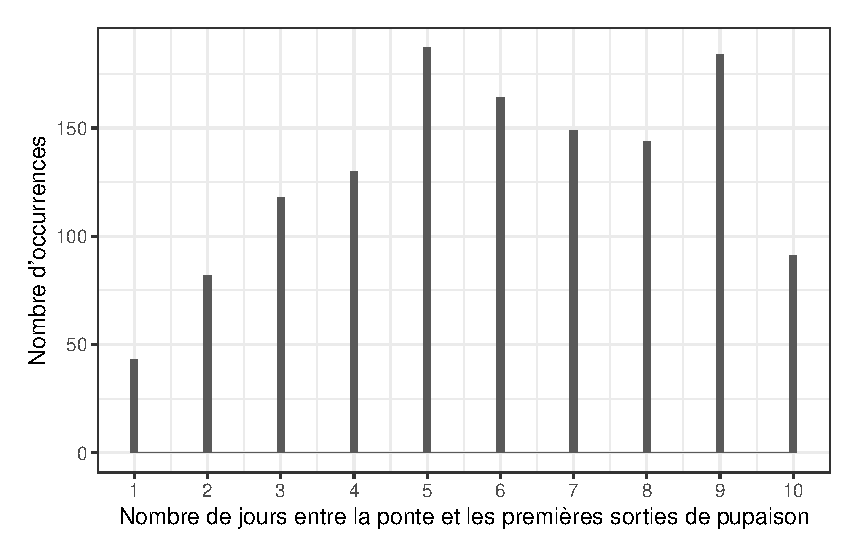
\epsfig{file = plots/duree_dvpmt.eps, scale = 0.6}
 \caption{Résultats de la calibration du premier jour d'enfouissement des larves après la ponte.}
 \label{fig:duree_dvpmt}
\end{figure}

Deux valeurs se dégagent légèrement des autres : 5 et 9 jours.
Lorsqu'on sélectionne une durée de développement larvaire qui est de 5 à 10 jours (\textit{i.e.} les résultats dont la durée de développement calibrée est égale à 5 contre 7 initialement), deux solutions--types apparaissent.
Elles sont visibles sur la figure~\ref{fig:E1}.

Les paramètres associés à la première sont :
\begin{center}
\small
\begin{tabular}{llllllll}
$\gamma$ & $p_{\text{m}}$ & $\mu_{\text{ER}}$ & $\mu_{\text{EH}}$ & $k$ & \texttt{stock} & $E_0\mu_\ell$ & premier jour d'enfouissement après la ponte\\
0.013 & 0.580 & 0.991 & 0.013 & 0.202 & 2112 & 6.759 & 5
 \end{tabular}
\end{center}
Cette solution ressemble à d'autres solutions trouvées par d'autres modèles où il n'y a pas beaucoup d'individus exogènes et où la sous-parcelle ER tient un rôle de fournisseur pour les deux autres sous-parcelles au détriment de la qualité d'ajustement.
On notera cependant que la qualité d'ajustement sur les deux autres sous-parcelles n'est pas bonne pour autant, les pics de larves estimées sont en avance sur les pics de larves observées, rendant la prédiction peu convaincante.

\begin{figure}[ht]
 \centering
 \textbf{Solution--type 1}
 
 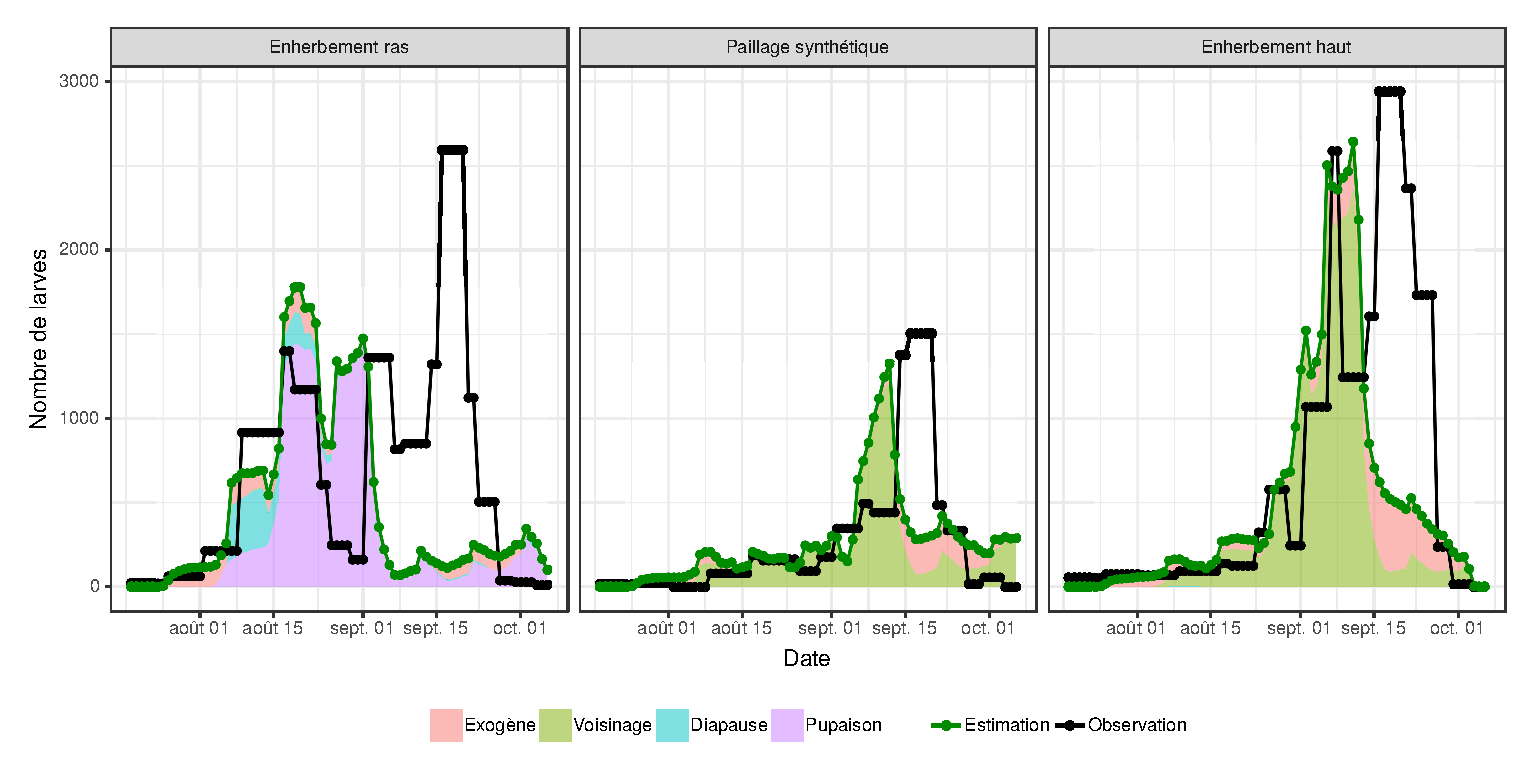
\epsfig{file = plots/E1.eps, scale = 0.52}
 
 \textbf{Solution--type 2}
 
 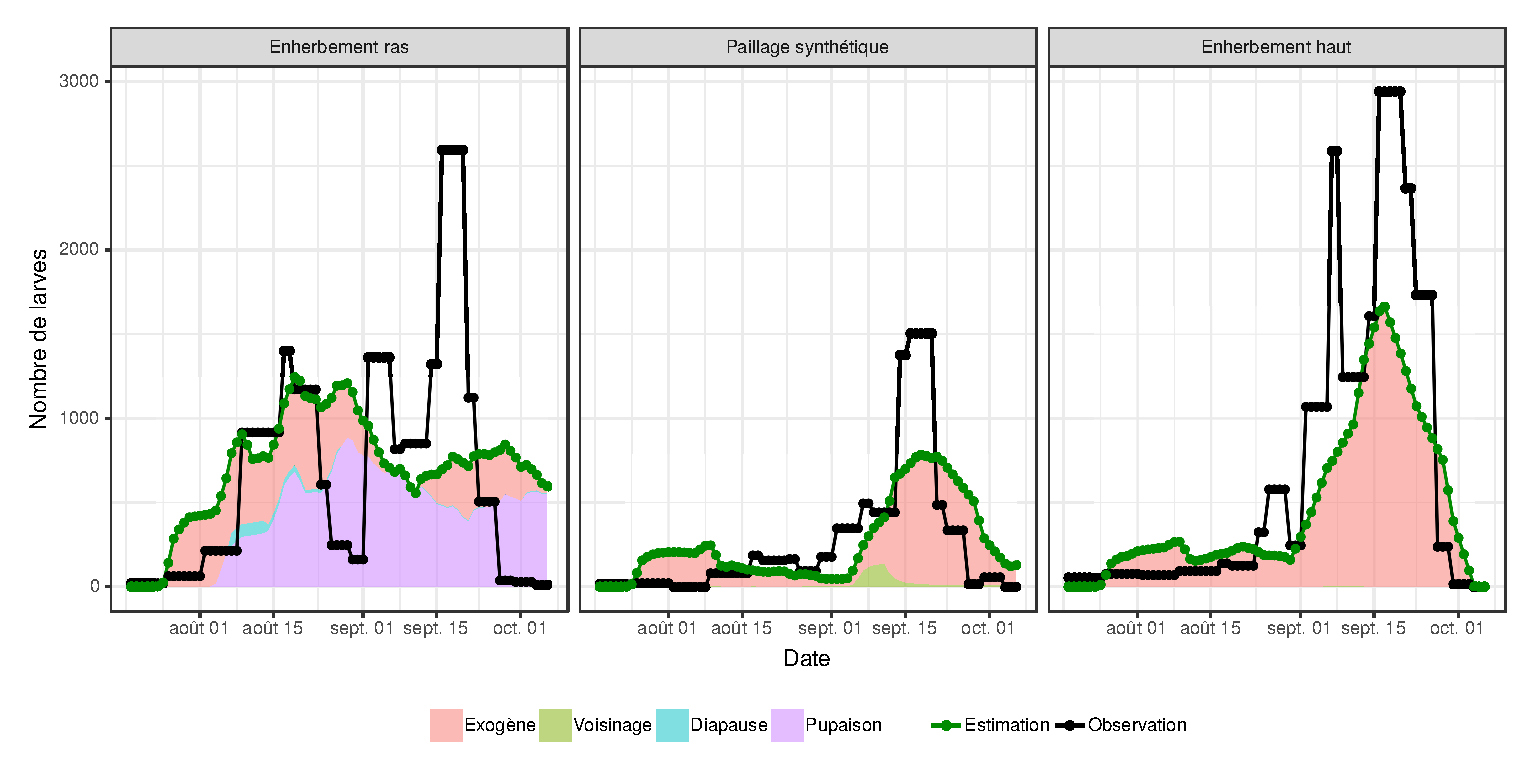
\epsfig{file = plots/E2.eps, scale = 0.52}
 \caption{Dynamiques observées et simulées pour chacune des deux solutions--types. La décomposition indiquant la provenance des femelles qui ont pondus les œufs est disponible pour les dynamiques simulées.}
 \label{fig:E1}
\end{figure}

La deuxième solution--type a pour paramètres
\begin{center}
\small
\begin{tabular}{llllllll}
$\gamma$ & $p_{\text{m}}$ & $\mu_{\text{ER}}$ & $\mu_{\text{EH}}$ & $k$ & \texttt{stock} & $E_0\mu_\ell$ & premier jour d'enfouissement après la ponte\\
0.030 & 0.013 & 0.421 & 0.007 & 1.278 & 509 & 10.72 & 5
 \end{tabular}
\end{center}
Dans cette prédiction, la synchronisation entre les pics de larves observées et estimées est présente.
Cependant, le modèle utilise beaucoup trop d'individus exogènes pour que cela soit acceptable.
En outre, la qualité d'ajustement sur la parcelle ER n'est pas bonne et celle sur les deux autres sous-parcelles est largement perfectible.

On s'intéresse à présent aux résultats qui ont une durée de développement larvaire comprise entre 9 et 14 jours (\textit{i.e.} une durée calibrée égale à 9).
On repère ici trois solutions--types, visibles sur la figure~\ref{fig:E3}.

\begin{figure}[ht]
 \centering
 \textbf{Solution--type 1}
 
 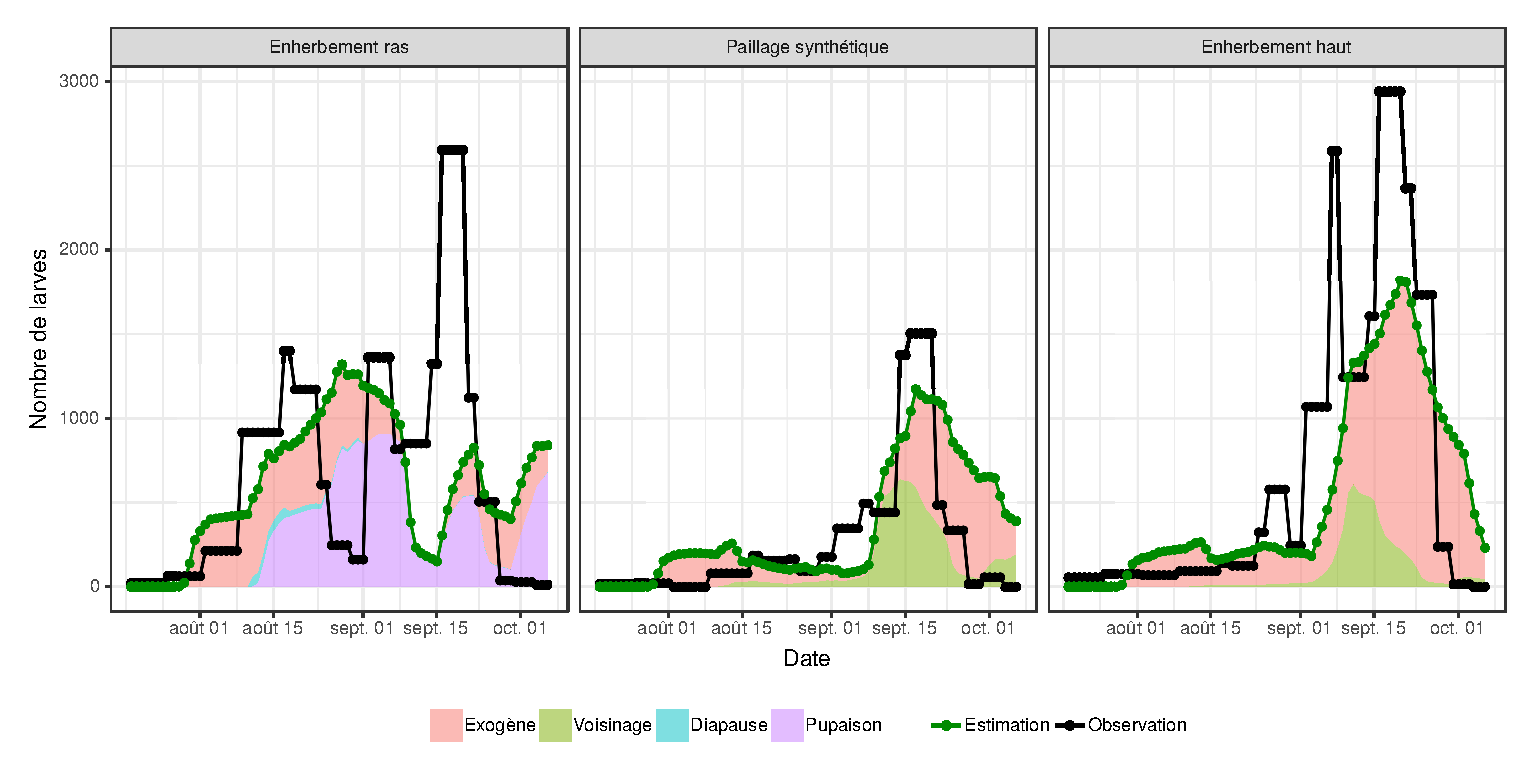
\epsfig{file = plots/E3.eps, scale = 0.52}
 
 \textbf{Solution--type 2}
 
 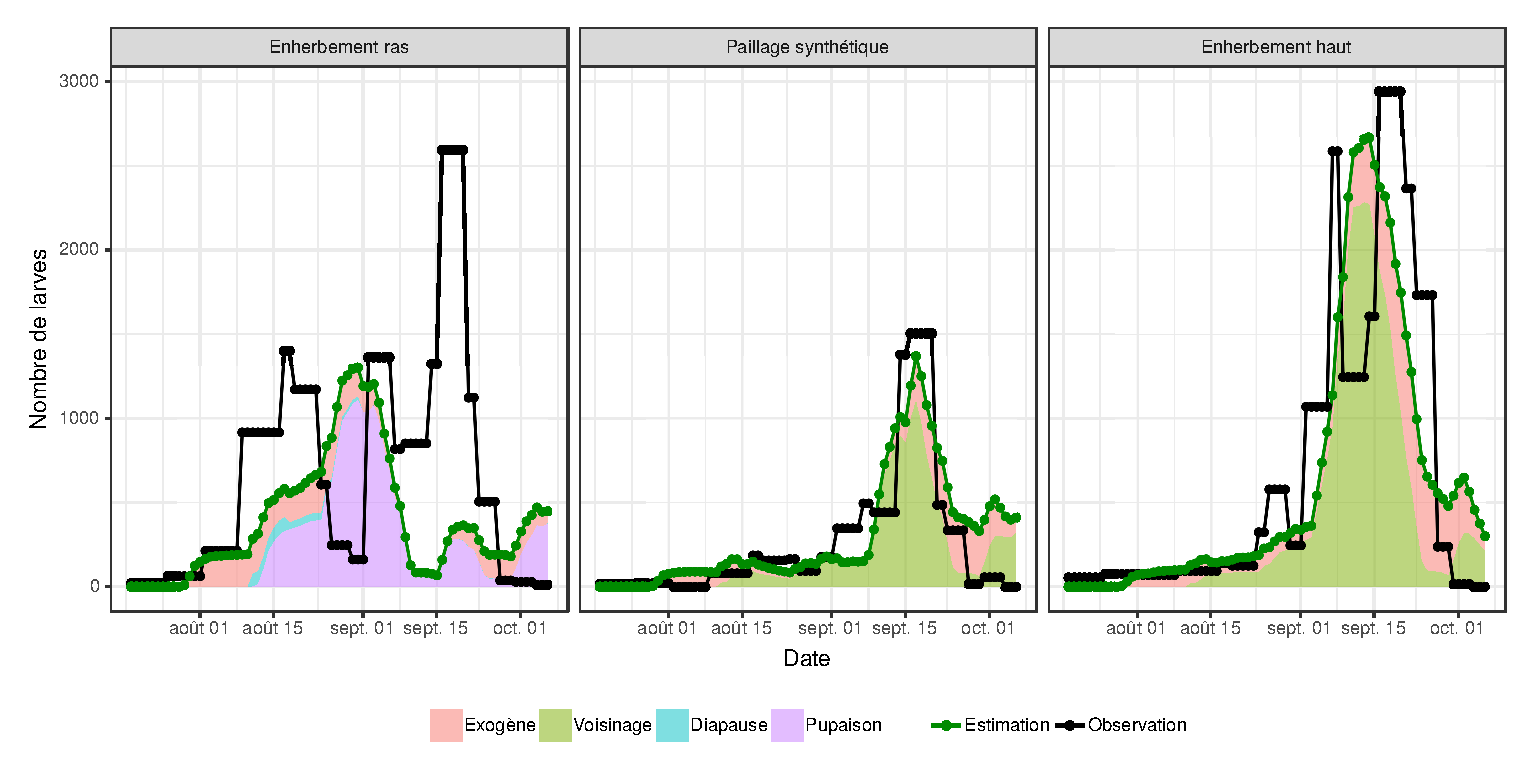
\epsfig{file = plots/E4.eps, scale = 0.52}
 
 \textbf{Solution--type 3}
 
 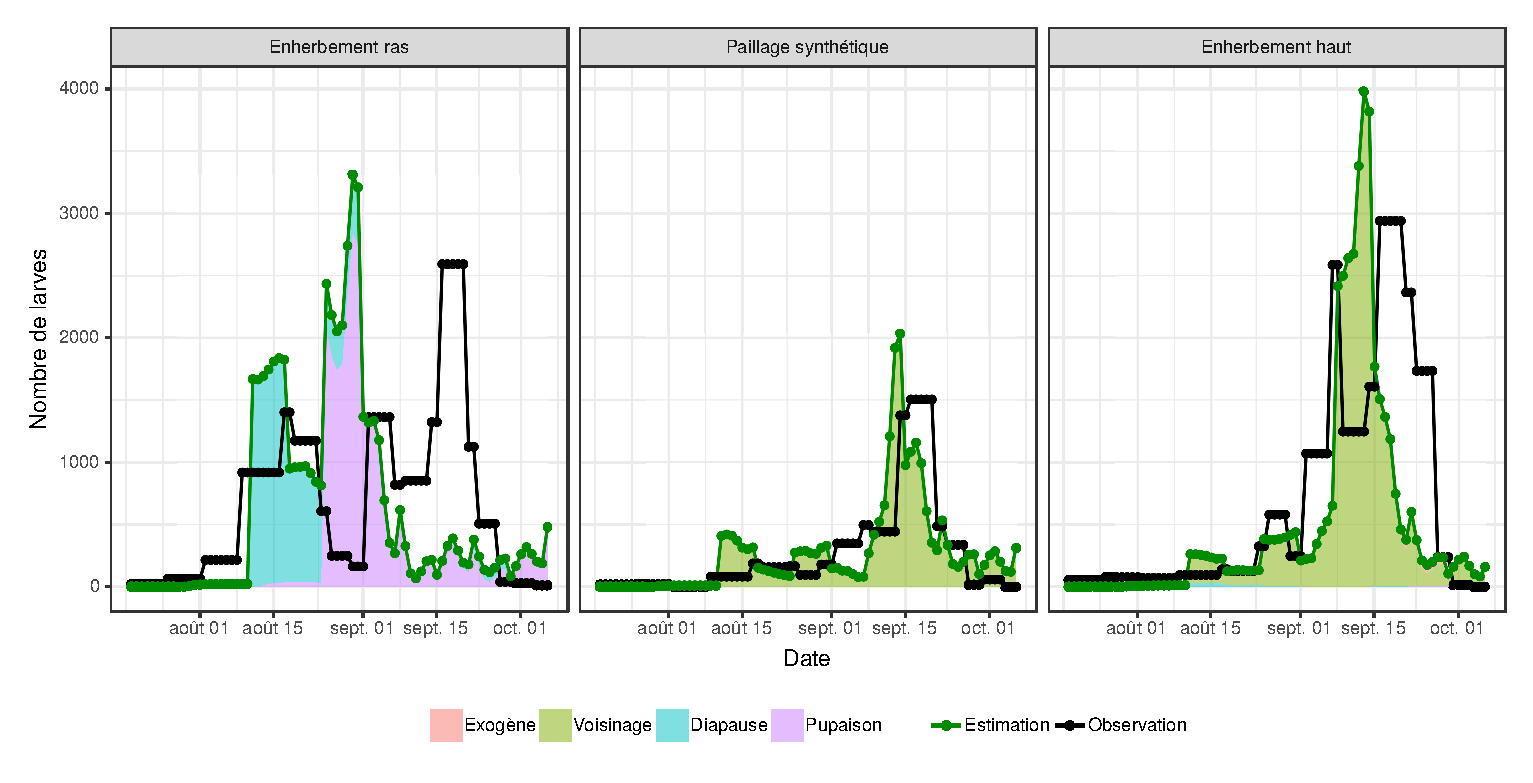
\epsfig{file = plots/E5.eps, scale = 0.52}
 \caption{Dynamiques observées et simulées pour chacune des trois solutions--types. La décomposition indiquant la provenance des femelles qui ont pondus les œufs est disponible pour les dynamiques simulées.}
 \label{fig:E3}
\end{figure}

La première de ces solutions a pour paramètres
\begin{center}
\small
\begin{tabular}{llllllll}
$\gamma$ & $p_{\text{m}}$ & $\mu_{\text{ER}}$ & $\mu_{\text{EH}}$ & $k$ & \texttt{stock} & $E_0\mu_\ell$ & premier jour d'enfouissement après la ponte\\
0.051 & 0.232 & 0.691 & 0.015 & 1.042 & 504 & 6.05 & 9
 \end{tabular}
\end{center}
On note une forte présence de femelles exogènes, avec des individus qui émergent uniquement de la sous-parcelle ER.
Des échanges sont présents mais plutôt restreints.
Relativement à d'autres solutions trouvées précédemment, cette solution--type semble peu pertinente.

La deuxième solution a pour paramètres
\begin{center}
\small
\begin{tabular}{llllllll}
$\gamma$ & $p_{\text{m}}$ & $\mu_{\text{ER}}$ & $\mu_{\text{EH}}$ & $k$ & \texttt{stock} & $E_0\mu_\ell$ & premier jour d'enfouissement après la ponte\\
0.018 & 0.698 & 0.941 & 0.001 & 0.211 & 501 & 7.693 & 9
 \end{tabular}
\end{center}
Cette solution semble être une variation de la précédente, à la différence que les individus exogènes serait peu nombreux. 
Les larves proviendrait donc de la sous-parcelle ER, qui servirait de «fournisseur» aux deux autres.
La qualité d'ajustement de la dynamique sur la sous-parcelle ER est mauvaise, et celle sur les deux autres est satisfaisante.
On peu cependant déplorer l'absence totale de femelles émergentes dans la sous-parcelle EH ($\mu_{\text{EH}} = 0.001$).

Enfin, la troisième solution--type a pour paramètres
\begin{center}
\small
\begin{tabular}{llllllll}
$\gamma$ & $p_{\text{m}}$ & $\mu_{\text{ER}}$ & $\mu_{\text{EH}}$ & $k$ & \texttt{stock} & $E_0\mu_\ell$ & premier jour d'enfouissement après la ponte\\
0.002 & 0.510 & 0.769 & 0.018 & 0.179 & 10159 & 8.686 & 9
 \end{tabular}
\end{center}
La solution présente ici est atypique dans la mesure où il n'y a pratiquement aucune femelles exogènes ($\gamma = 0.002$) et que ce sont les individus issus de la diapause qui lance la dynamique.
On notera l'absence d'individus qui émergent de la sous-parcelle EH.
Les dynamiques sur les sous-parcelles PS et EH sont bonnes.
Celle sur la sous-parcelle ER n'est pas excellente mais a le mérite de présenter deux pics distincts comme sur les données observées.



% Une valeur se dégage légèrement des autres : 5 jours.
% Cependant, les solutions--types dont l'émergence des individus en pupaison débute 5 jours après la ponte des œufs ne sont pas très bonnes en comparaison de solutions trouvés par d'autres modèles.
% Une des meilleures prédictions est visible sur la figure~\ref{fig:duree_dvpmt2}, les paramètres associés sont :
% \begin{center}
% \small
% \begin{tabular}{llllllll}
% $\gamma$ & $p_{\text{m}}$ & $\mu_{\text{ER}}$ & $\mu_{\text{EH}}$ & $k$ & \texttt{stock} & $E_0\mu_\ell$ & premier jour d'émergence après la ponte\\
% 0.095 & 0.154 & 0.880 & 0.104 & 1.995 & 531 & 3.212 & 5
%  \end{tabular}
% \end{center}
% Comme l'on peut le voir, les dynamiques ne sont pas bien captées et les femelles sont surtout exogènes : cette solution--type n'est pas convaincante.
% 
% \begin{figure}[ht]
%  \centering
%  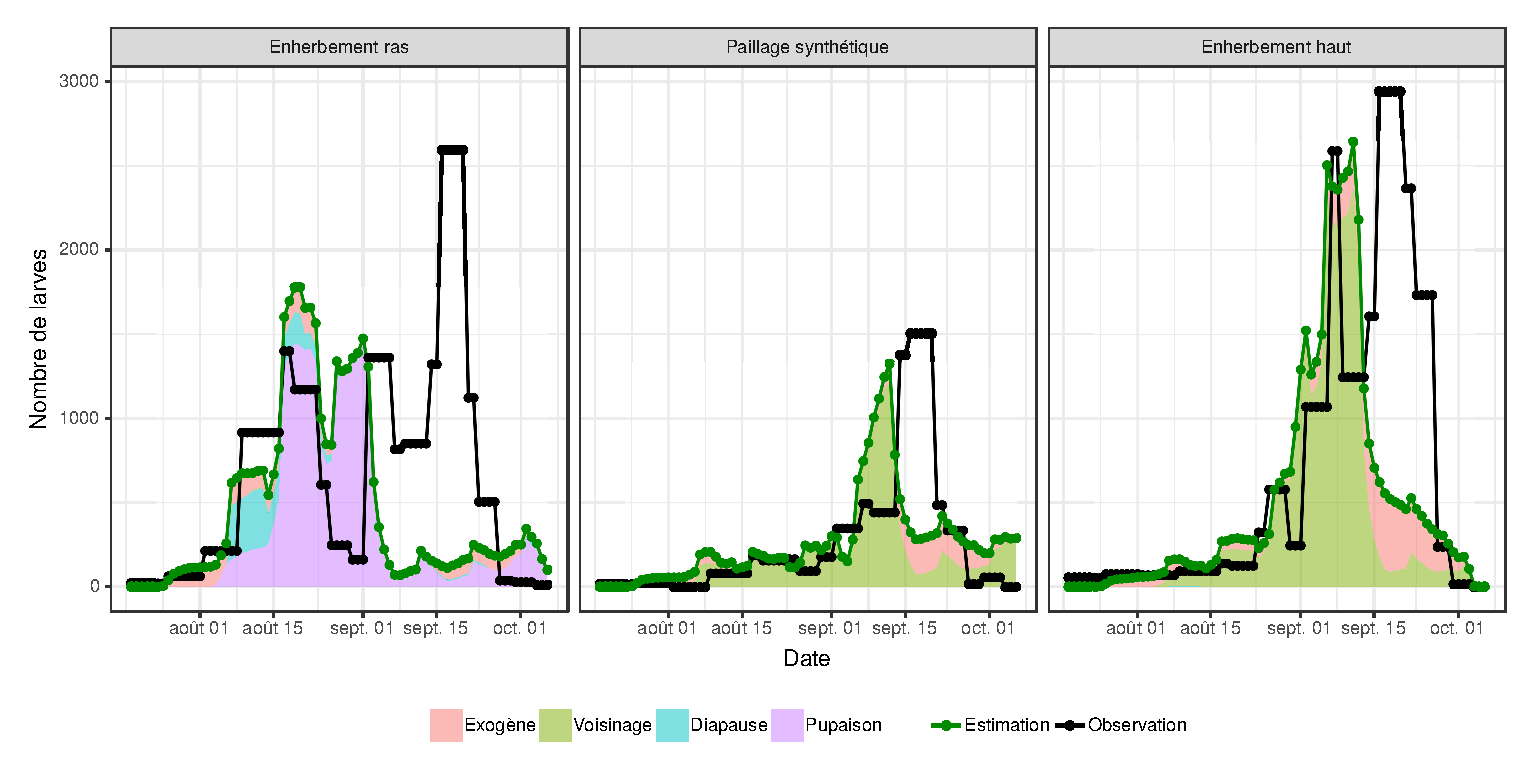
\epsfig{file = plots/E1.eps, scale = 0.57}
%  \caption{Dynamiques observées et simulées. La décomposition indiquant la provenance des femelles qui ont pondus les œufs est disponible pour les dynamiques simulées.}
%  \label{fig:duree_dvpmt2}
% \end{figure}
% 
% On s'intéresse aussi au jeux de paramètres dont l'enfouissement des larves dans le sol a lieu deux ou trois jours après la ponte.


% Simu
\chapter{Simulations} 

Cette annexe a pour but de tester l'impact de la distribution des inflorescences en entrée d'une version du modèle donnée sur le nombre de larves total prédit trouvés par celle-ci.

Pour faire cela, on se donne deux dynamiques d'inflorescences différentes : l'une ne possède qu'un seul \textit{flush}, l'autre en possède deux (voir figure~\ref{fig:flush}). 
Il est important de noter que le nombre d'inflorescences considérées sera identique pour les deux dynamiques, sans quoi comparer le nombre de larves ne serait pas pertinent.

\begin{figure}[h]
 \centering
 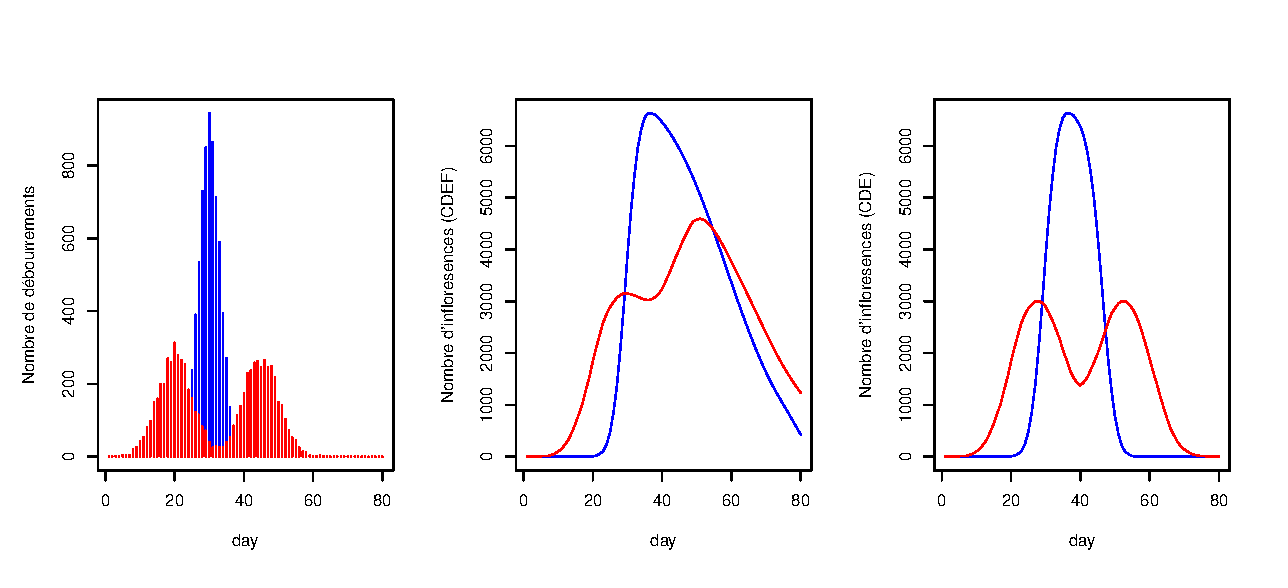
\epsfig{file = plots/dynamiques.eps, scale = 0.7}
 \caption{Représentation des dynamiques d'inflorescences simulées vivantes (au milieu) ou aux stades phénologiques C, D et E (à droite) avec les débourrements correspondants (à gauche). }
 \label{fig:flush}
\end{figure}

Pour être raccord avec ce qui a été fait précédemment, on utilisera les inflorescences vivantes (aux stades C, D, E et F) dès lors que l'on utilisera le modèle A, et les inflorescences aux stades phénologiques C, D et E lorsque l'on utilisera les modèles C ou D.

\section{Modèle A}

On s'intéresse aux résultats obtenus en utilisant les jeux de paramètres correspondant aux deux premières solutions--types trouvées (la troisième ne nous semble pas pertinente).
Les résultats pour la première solution--type sont :
{%
\newcommand{\mc}[3]{\multicolumn{#1}{#2}{#3}}
\begin{center}
\begin{tabular}{lllllll}
\mc{7}{c}{\textbf{Paramètres}}\\
$\gamma$ & $p_{\text{m}}$ & $\mu_{\text{ER}}$ & $\mu_{\text{EH}}$ & $k$ & \texttt{stock} & $E_0\mu_{\ell}$\\
0.08 & 0.494 & 0.976 & 0.046 & 1.928 & 5600 & 3.084\\\hline
\mc{2}{r}{ } & \mc{5}{r}{Nombre de larves total}\\
\mc{2}{r}{1 flush} & \mc{5}{r}{216 204}\\
\mc{2}{r}{2 flushs} & \mc{5}{r}{206 048}
\end{tabular}
\end{center}
}%
Les résultats pour la deuxième solution--type sont :
{%
\newcommand{\mc}[3]{\multicolumn{#1}{#2}{#3}}
\begin{center}
\begin{tabular}{lllllll}
\mc{7}{c}{\textbf{Paramètres}}\\
$\gamma$ & $p_{\text{m}}$ & $\mu_{\text{ER}}$ & $\mu_{\text{EH}}$ & $k$ & \texttt{stock} & $E_0\mu_{\ell}$\\
0.000 & 0.968 & 1.000 & 0.025 & 0.100 & 14483 & 6.260\\\hline
\mc{2}{r}{ } & \mc{5}{r}{Nombre de larves total}\\
\mc{2}{r}{1 flush} & \mc{5}{r}{37 079}\\
\mc{2}{r}{2 flushs} & \mc{5}{r}{100 018}
\end{tabular}
\end{center}
}%

Au vu des deux résultats, il est difficile de proposer une interprétation tant aucune tendance ne semble se dégager lorsqu'on l'on change de jeu de paramètres.

\section{Modèle C}

On réitère en utilisant le modèle C qui semblait obtenir des résultats plus pertinent.
Les résultats pour la première solution--type sont :
{%
\newcommand{\mc}[3]{\multicolumn{#1}{#2}{#3}}
\begin{center}
\begin{tabular}{lllllll}
\mc{7}{c}{\textbf{Paramètres}}\\
$\gamma$ & $p_{\text{m}}$ & $\mu_{\text{ER}}$ & $\mu_{\text{EH}}$ & $k$ & \texttt{stock} & $E_0\mu_{\ell}$\\
0.115 & 0.189 & 0.898 & 0.012 & 1.877 & 515 & 3.097\\\hline
\mc{2}{r}{ } & \mc{5}{r}{Nombre de larves total}\\
\mc{2}{r}{1 flush} & \mc{5}{r}{140 138}\\
\mc{2}{r}{2 flushs} & \mc{5}{r}{170 557}
\end{tabular}
\end{center}
}%

Les résultats pour la deuxième solution--type sont :
{%
\newcommand{\mc}[3]{\multicolumn{#1}{#2}{#3}}
\begin{center}
\begin{tabular}{lllllll}
\mc{7}{c}{\textbf{Paramètres}}\\
$\gamma$ & $p_{\text{m}}$ & $\mu_{\text{ER}}$ & $\mu_{\text{EH}}$ & $k$ & \texttt{stock} & $E_0\mu_{\ell}$\\
0.004 & 0.490 & 0.990 & 0.018 & 0.242 & 9970 & 5.638\\\hline
\mc{2}{r}{ } & \mc{5}{r}{Nombre de larves total}\\
\mc{2}{r}{1 flush} & \mc{5}{r}{29 764}\\
\mc{2}{r}{2 flushs} & \mc{5}{r}{122 692}
\end{tabular}
\end{center}
}%

Ici une tendance se dégage : il y a moins de larves lorsque la dynamique de floraison ne présente qu'un seul \textit{flush}.
On peut remarquer que la diminution est d'autant plus forte lorsque le modèle ne fait appel qu'à peu d'individus exogènes

\section{Modèle D}

On s'intéresse à présent au modèle D, qui comprend un phénomène de saisonnalité.
Les résultats pour la première solution--type sont :
{%
\newcommand{\mc}[3]{\multicolumn{#1}{#2}{#3}}
\begin{center}
\begin{tabular}{llllllll}
\mc{8}{c}{\textbf{Paramètres}}\\
$\gamma$ & $p_{\text{m}}$ & $\mu_{\text{ER}}$ & $\mu_{\text{EH}}$ & $k$ & \texttt{stock} & $E_0\mu_{\ell}$ & $\xi$\\
0.021 & 0.105 & 0.938 & 0.916 & 1.992 & 516 & 6.018 & 0.004\\\hline
\mc{2}{r}{ } & \mc{6}{r}{Nombre de larves total}\\
\mc{2}{r}{1 flush} & \mc{6}{r}{81 073}\\
\mc{2}{r}{2 flushs} & \mc{6}{r}{113 068}
\end{tabular}
\end{center}
}%

Les résultats pour la deuxième solution--type sont :
{%
\newcommand{\mc}[3]{\multicolumn{#1}{#2}{#3}}
\begin{center}
\begin{tabular}{llllllll}
\mc{8}{c}{\textbf{Paramètres}}\\
$\gamma$ & $p_{\text{m}}$ & $\mu_{\text{ER}}$ & $\mu_{\text{EH}}$ & $k$ & \texttt{stock} & $E_0\mu_{\ell}$ & $\xi$\\
0.019 & 0.131 & 0.999 & 0.743 & 0.262 & 508 & 6.190 & 0.060\\\hline
\mc{2}{r}{ } & \mc{6}{r}{Nombre de larves total}\\
\mc{2}{r}{1 flush} & \mc{6}{r}{63 686}\\
\mc{2}{r}{2 flushs} & \mc{6}{r}{104 882}
\end{tabular}
\end{center}
}%

La même tendance que pour le modèle C se dégage : une dynamique de floraison avec un unique \textit{flush} semble limiter la présence de larves.


\end{document}

